\documentclass[10pt]{article}
\usepackage[a4paper,margin=0.5in]{geometry}
\usepackage{graphicx}
\usepackage{amsmath,amssymb,latexsym}
\usepackage{mathpartir}
\usepackage{../lstnicec}
\usepackage{../threadq}
\usepackage{hyperref}

\parindent=0pt % I hate first line indentation
\parskip=3pt   % I like a visual white gap between paragraphs
% \def\rulebefore{\vspace{-6pt}\\\rule{\textwidth}{0.1pt}\vspace{-10pt}}
% \def\ruleafter{\vspace{-16pt}\rule{\textwidth}{0.1pt}\\}
% \newenvironment{code}%
%   {~\rulebefore\small\verbatim}%
%   {\endverbatim\normalsize\ruleafter}


\author{Andrew Butterfield}
\title{Notes: RTEMS-SMP Thread Queues}
\date\today

\begin{document}
\maketitle
\tableofcontents

\newpage\section{Introduction}

Here we record various notes about the RTEMS-SMP Thread Queue implementation.

\textbf{Note:}
\textsf{some of these notes are just cut-and-paste from authoritative sources,
and are not intended for use as-is in any publication.} 

\newpage\section{Classic User Manual Notes}

Notes from
``RTEMS Classic API Guide'',
Release 6.66bcecf (2nd December 2020).

\newpage\subsection{Chapter 3 Key Concepts}

\subsubsection{Thread Queues}

p28:

Binary semaphores may utilize the optional priority
inheritance algorithm to avoid the problem of priority inversion.

p29:

RTEMS supports the four locking protocols (ICPP,PIP,MrsP,OMIP)
for synchronization objects providing mutual-exclusion (mutex).

One aim of the
locking protocols is to avoid priority inversion.

priority updates due to the locking protocols take place immediately and are
propagated recursively.
The mutex owner and wait for mutex relationships define a directed
acyclic graph (DAG).
The run-time of the mutex obtain, release and timeout operations depend
on the complexity of this resource dependency graph.

Priority inversion occurs when a high priority tasks
requests access to shared resource
which is currently allocated to a low priority task.

\dots
the low priority task is prevented from executing by one or more medium priority
tasks.

Although the priority ceiling protocol is
more efficient than the priority inheritance protocol
with respect to the maximum number of
thread priority changes which may occur
while a thread owns a particular mutex,
the priority inheritance protocol is more forgiving
in that it does not require this apriori information.

p30:

priority updates due to the priority
inheritance protocol take place immediately and are propagated recursively.

This means the
priority inheritance is transitive

If a task A owning a priority inheritance
mutex blocks on another priority inheritance mutex, then the owner of this mutex inherits the
priority of the task A.

Threads that wait for mutex ownership are not blocked
with respect to the scheduler and instead
perform a busy wait.

The complex part of the implementation is contained in the thread
queues and shared with the MrsP support.

p31:

Threads can wait in FIFO or priority order.

It makes
no sense to compare the priority values of two different scheduler instances.

The top-level queue provides FIFO ordering
and contains priority queues.
Each priority queue is associated with a scheduler instance and
contains only threads of this scheduler instance.
Threads are enqueued in the priority queues
corresponding to their scheduler instances.
To dequeue a thread, the highest priority thread of
the first priority queue is selected.
Once this is done, the first priority queue is appended to the
top-level FIFO queue.

\textbf{The following excerpt is a bit head-wrecking and needs some thought}

\begin{quote}
``
Such a two-level queue needs a considerable amount of memory
if fast enqueue and dequeue
operations are desired.
Providing this storage per thread queue would waste a lot of memory
in typical applications.
Instead, each thread has a queue attached which resides in a dedicated
memory space independent of other memory
used for the thread (this approach was borrowed
from FreeBSD).
In case a thread needs to block, there are two options
\begin{itemize}
  \item
    the object already has a queue,
    then the thread enqueues itself to this already present queue
    and the queue of the thread is added to
    a list of free queues for this object, or
  \item
    otherwise,
    the queue of the thread is given to the object
    and the thread enqueues itself to this queue.
\end{itemize}
In case the thread is dequeued, there are two options
\begin{itemize}
  \item
    the thread is the last thread in the queue,
    then it removes this queue from the object and
    reclaims it for its own purpose, or
  \item
    otherwise,
    the thread removes one queue from the free list of the object
    and reclaims it for its own purpose.
\end{itemize}
Since there are usually more objects than threads, this actually reduces the memory demands.
In addition the objects only contain a pointer to the queue structure. This helps to hide implementation
details. Inter-cluster priority queues are available since RTEMS 5.1.
''
\end{quote}

A doubly-linked list (chain) is used to implement the FIFO queues
yielding a $O(1)$ worst-case
time complexity for enqueue and dequeue operations.

A red-black tree is used to implement the priority queues
yielding a $O(\log(n))$ worst-case time
complexity for enqueue and dequeue operations
with $n$ being the count of threads already on
the queue.

\newpage\subsection{Chapter 5 Scheduling Concepts}

\subsubsection{Introduction}

p42:

The scheduler’s sole purpose is to allocate
the  all important resource of processor time
to the various tasks competing for attention.

\subsubsection{Background}

p43:

Priority based scheduling algorithms will always select
the highest priority task that is ready to run
when allocating the processor to a task.

There are a few common methods of accomplishing the mechanics of this algorithm.
These ways involve a list or chain of tasks in the ready state.

p43--44:

Another mechanism is to maintain a list of FIFOs per priority.
When a task is readied,
it is placed on the rear of the FIFO for its priority.
This method is often used with a bitmap to assist in locating
which FIFOs have ready tasks on them.
This data structure has $O(1)$ insert, extract
and find highest ready run-time complexities.

p44:

A red-black tree may be used for the ready queue with the priority as the key.
This data structure has $O(\log(n))$ insert, extract
and find highest ready run-time complexities
while $n$ is the count of tasks in the ready queue.

RTEMS provides four mechanisms which allow the user to alter the task scheduling decisions:
\begin{itemize}
  \item
    user-selectable task priority level
  \item
    task preemption control
  \item
    task timeslicing control
  \item
    manual round-robin selection
\end{itemize}

The evaluation order for scheduling characteristics is always
priority, preemption mode, and timeslicing.

A lower priority level means higher priority (higher importance).

Note that the preemption setting has no effect
on the manner in which a task is scheduled.
It only applies once a task has control of the processor.

p46:

Tasks in an RTEMS system must always be in
one of the five allowable task states.
These states are: executing, ready, blocked, dormant, and non-existent.

State Diagram:
\begin{eqnarray*}
   NonExistent  &\defs&  create      \then Dormant
\\ Dormant      &\defs&  deleting    \then NonExistent
                         \extc
                         starting    \then Ready
\\ Ready       &\defs&   deleting    \then NonExistent
                         \extc
                         dispatching \then Executing
                         \extc
                         blocking    \then Blocked
\\ Executing   &\defs&   deleting    \then NonExistent
                         \extc
                         yielding    \then Ready
                         \extc
                         blocking    \then Blocked
\\ Blocked     &\defs&   deleting    \then NonExistent
                         \extc
                         readying    \then Ready
\end{eqnarray*}

p47:

A blocked task may also be suspended.
Therefore,
both the suspension and the blocking condition must be removed
before the task becomes ready to run again.

\subsubsection{Uniprocessor Schedulers}

p49:

5.3.1 Deterministic Priority Scheduler
\dots
It schedules tasks using a priority based algorithm
which takes into account preemption.
\dots
an array of FIFOs with a FIFO per priority.
a bitmap which is used to track which priorities have ready tasks.
\dots
deterministic (e.g., predictable and fixed) in execution time.

\textit{More single-core scheduler descriptions follow\dots}

\subsubsection{SMP Schedulers}

p51:

All SMP schedulers included in RTEMS are priority based.

\paragraph{Earliest Deadline First SMP Scheduler}

job-level fixed-priority scheduler using the Earliest Deadline First

supports \emph{task processor affinities}
of one-to-one and one-to-all, e.g., a task can execute on exactly one processor
or all processors managed by the scheduler instance.

The processor affinity set of a task must
contain all online processors to select the one-to-all affinity.

supports \emph{thread pinning}

ready queues use a red-black tree with the task priority as the key.

\paragraph{Deterministic Priority SMP Scheduler}

A fixed-priority scheduler which uses a table of chains
with one chain per priority level for the ready tasks.

\paragraph{Simple Priority SMP Scheduler}

A fixed-priority scheduler which uses a sorted chain for the ready tasks.

\paragraph{Arbitrary Processor Affinity Priority SMP Scheduler}

A fixed-priority scheduler which uses a table of chains with one chain per priority level for the
ready tasks.

This scheduler supports arbitrary task processor affinities

\newpage\subsection{Chapter 8 Interrupt Manager}

\subsubsection{Introduction}

p120:

This manager permits quick interrupt response times by
providing the critical ability to alter task execution
which allows a task to be preempted upon exit from an ISR.

\subsubsection{Background}

p121:

The interrupt manager allows the application to connect a function
to a hardware interrupt vector.
When an interrupt occurs,
the processor will automatically vector to RTEMS.
RTEMS saves and restores all registers which are not preserved
by the normal C calling convention for the target processor
and invokes the user’s ISR.
The user’s ISR is responsible for processing the interrupt,
clearing the interrupt if necessary,
and device specific manipulation.

The \verb"rtems_interrupt_catch" directive
connects a procedure to an interrupt vector.
The vector number is managed using the \verb"rtems_vector_number" data type.

The interrupt service routine is assumed to abide by these conventions
and have a prototype similar to the following:

\begin{nicec}
rtems_isr user_isr(
  rtems_vector_number vector
);
\end{nicec}

Once the user’s ISR has completed,
it returns control to the RTEMS interrupt manager
which will perform task dispatching
and restore the registers saved before the ISR was invoked.

A system call made by the ISR may have readied a task of
higher priority than the interrupted task.

No dispatch processing is performed as part of directives
which have been invoked by an ISR.

Applications must adhere to the following rule if proper task scheduling and dispatching is to
be performed:

\textbf{Note:} \textit{The interrupt manager must be used for all ISRs which may be interrupted by the highest
priority ISR which invokes an RTEMS directive.}

Interrupts are nested whenever an interrupt occurs during the execution of another ISR. RTEMS
supports efficient interrupt nesting by allowing the nested ISRs to terminate without performing
any dispatch processing. Only when the outermost ISR terminates will the postponed dispatching
occur.

p122:

During the execution of directive calls,
critical sections of code may be executed.
When these sections are encountered,
RTEMS disables all maskable interrupts
before the execution of the section
and restores them to the previous level upon completion of the section.

Non-maskable interrupts (NMI) cannot be disabled,
and ISRs which execute at this level MUST NEVER issue RTEMS system calls.

However,
ISRs that make no system calls may safely execute as non-maskable interrupts.

\subsubsection{Operations}

p123:

8.3.2 Directives Allowed from an ISR

Directives invoked by an ISR must operate only on objects
which reside on the local node.

\newpage\subsection{Chapter 12 Semaphore Manager}

\subsubsection{Introduction}

p206:

The semaphore manager utilizes standard Dijkstra counting semaphores
to provide synchronization and mutual exclusion capabilities.

\subsubsection{Background}

p207:

A binary semaphore (not a simple binary semaphore)
can be used to control access to a single resource.
\dots
In this instance, the semaphore would be created with an initial count of one to
indicate that no task is executing the critical section of code.

A binary semaphore must be released by the task that obtained it.

A counting semaphore can be used to control access
to a pool of two or more resources.
\dots
access to three printers could be administered by a semaphore
created with an initial count of three.

Task synchronization may be achieved by creating a semaphore
with an initial count of zero.

Simple binary semaphores do not allow nested access
and so can be used for task synchronization.

p208:

\verb"RTEMS_SIMPLE_BINARY_SEMAPHORE":
restrict values to 0 and 1,
do not allow nested access,
allow deletion of locked semaphore.

p209:

Some combinatinos\emph{(sic.)} of these attributes are invalid.

The following tree figure illustrates the valid combinations.

Classic Semaphore
$\mapsto \{$
 Counting Semaphore; Simple Binary; Binary (Mutex)
$\}$

Counting Semaphore
$\mapsto \{$
 FIFO; Priority
$\}$

Simple Binary
$\mapsto \{$
 FIFO; Priority
$\}$

Binary (Mutex)
$\mapsto \{$
 FIFO; Priority
$\}$

Binary (Mutex)
$\mapsto \{$
 Priority
 $\mapsto \{$
   No Protocol; Priority Inheritance Protocol; Priority Ceiling Protocol
 $\}$
$\}$

\subsubsection{Operations}

\paragraph{Creating a Semaphore}

p210:

If a binary semaphore is created with a count of zero (0)
to indicate that it has been allocated,
then the task creating the semaphore
is considered the current holder of the semaphore.

RTEMS allocates a Semaphore Control Block (SMCB) from the SMCB free list.

\paragraph{Obtaining Semaphore IDs}

\paragraph{Acquiring a Semaphore}

If the semaphore’s count is greater than zero
then decrement the semaphore’s count
else wait for release of semaphore then return SUCCESSFUL.

If the task blocked waiting for a binary semaphore
using priority inheritance
and the task’s priority is greater than that of
the task currently holding the semaphore,
then the holding task will inherit the priority of the blocking task.

When a task successfully obtains a semaphore using priority ceiling
and the priority ceiling for this semaphore is greater than that of the holder,
then the holder’s priority will be elevated.

\paragraph{Releasing a Semaphore}

p211:

If there are no tasks are waiting on this semaphore
then increment the semaphore’s count
else assign semaphore to a waiting task and return SUCCESSFUL.

If this is the outermost release of a binary semaphore
that uses priority inheritance or priority ceiling
and the task does not currently hold any other binary semaphores,
then the task performing the \verb"rtems_semaphore_release"
will have its priority restored to its normal value.

\paragraph{Deleting a Semaphore}

As a result of this directive,
all tasks blocked waiting to acquire the semaphore
will be readied
and returned a status code which indicates that the semaphore was deleted.

\newpage\subsection{Chapter 26 Multiprocessing Manager}

\textbf{Note:}
\textsf{
At the weekly meeting of 16th March 2021,
Sebastian Huber said that this Manager is to be
considered deprecated,
and that the ``node'' concept no longer really applies,
and has been replaced in the SMP enhancements by the
notion of ``processor''.
}

\subsubsection{Introduction}

p514:

RTEMS allows the entire system,
both hardware and software,
to be viewed logically as a single system.

\subsubsection{Background}

p515:

In keeping with RTEMS philosophy
of providing transparent physical node boundaries,
the minimal heterogeneous processing required is isolated in the MPCI layer.

A processor in a RTEMS system is referred to as a node.
Each node is assigned a unique nonzero node number by the application designer.
RTEMS assumes that node numbers are assigned consecutively
from one to the \verb"maximum_nodes" configuration parameter.

RTEMS assumes that node numbers are assigned
consecutively from one to the \verb"maximum_nodes" configuration parameter.

The Multiprocessor Communications Interface Layer (MPCI)
must be able to route messages based on the node number.

All RTEMS objects which are created with the GLOBAL attribute
will be known on all other nodes.

A task does not have to be global
to perform operations involving remote objects.

The distribution of tasks to processors is performed
during the application design phase.
Dynamic task relocation is not supported by RTEMS.

p516:

RTEMS maintains two tables containing object information
on every node in a multiprocessor system:
a local object table and a global object table.
The local object table on each node is unique
and contains information for all objects created on this node
whether those objects are local or global.
The global object table contains information regarding
all global objects in the system and, consequently, is the same on every node.

To maintain consistency among the table copies,
every node in the system must be informed
of the creation or deletion of a global object.

When an application performs an operation on a remote global object,
RTEMS must generate a Remote Request (RQ) message
and send it to the appropriate node.
After completing the requested operation,
the remote node will build a Remote Response (RR) message
and send it to the originating node.
Messages generated as a side-effect of a directive
(such as deleting a global task)
are known as Remote Processes (RP)
and do not require the receiving node to respond.

p517:

If an uncorrectable error occurs in the user-provided MPCI layer,
the fatal error handler should be invoked.
RTEMS assumes the reliable transmission and reception of messages
by the MPCI and makes no attempt to detect or correct errors.

A proxy is an RTEMS data structure which resides on a remote node
and is used to represent a task which must block as part of a remote operation.
This action can occur as part of the \verb"rtems_semaphore_obtain"
and \verb"rtems_message_queue_receive" directives.
If the object were local,
the task’s control block would be available for modification
to indicate it was blocking on a message queue or semaphore.
However,
the task’s control block resides only on the same node as the task.
As a result,
the remote node must allocate a proxy to represent the task
until it can be readied.

\subsubsection{Multiprocessor Communications Interface Layer}

p518:

The Multiprocessor Communications Interface Layer (MPCI)
is a set of user-provided procedures
which enable the nodes in a multiprocessor system
to communicate with one another.

A packet is sent by RTEMS in each of the following situations:
\begin{itemize}
  \item an RQ is generated on an originating node;
  \item an RR is generated on a destination node;
  \item a global object is created;
  \item a global object is deleted;
  \item a local task blocked on a remote object is deleted;
  \item during system initialization to check for system consistency.
\end{itemize}

\subsubsection{Operations}


p522:

The \verb"rtems_multiprocessing_announce" directive is called by the MPCI layer
to inform RTEMS that a packet has arrived from another node.
This directive can be called from
an interrupt service routine
or from within a polling routine.

\newpage\subsection{Chapter 27 SYMMETRIC MULTIPROCESSING (SMP)}

\subsubsection{Introduction}

p526:

The RTEMS interpretation of real-time on SMP
is the support for Clustered Scheduling
with priority based schedulers and adequate locking protocols.

\subsubsection{Background}

pp527--8:

In an SMP system with N processors,
these are the new execution characteristics.
\begin{itemize}
  \item N tasks execute in parallel
  \item hardware events result in interrupts
\end{itemize}
There is true parallelism with a task executing on each processor
and the possibility of interrupts occurring on each processor.
Thus in contrast to their being one task and one interrupt
to consider on a uniprocessor,
there are N tasks and potentially N simultaneous interrupts
to consider on an SMP system.

p528:

Affinity is used to specify the subset of processors
in an SMP system on which a particular task can execute.

Only a subset of the available schedulers support affinity.

The scheduler with support for arbitary processor affinities
uses a proof of concept implementation.
See \url{https://devel.rtems.org/ticket/2510}
(this ticket is worth re-reading at some stage!).

With more than one processor in the system tasks can migrate from one processor to another.
There are four reasons why tasks migrate in RTEMS.
\begin{itemize}
  \item
    The scheduler changes explicitly
    via \verb"rtems_task_set_scheduler()" or similar directives.
  \item
    The task processor affinity changes explicitly
    via \verb"rtems_task_set_affinity()" or similar directives.
  \item
    The task resumes execution after a blocking operation.
    On a priority based scheduler it will evict
    the lowest priority task
    currently assigned to a processor in the processor set
    managed by the scheduler instance.
  \item
    The task moves temporarily to another scheduler instance
    due to locking protocols like
    the \emph{Multiprocessor Resource Sharing Protocol (MrsP)}
    or the \emph{O(m) Independence-Preserving Protocol (OMIP)}.
\end{itemize}

p529:

We have clustered scheduling in case
the set of processors of a system is partitioned
into nonempty pairwise-disjoint subsets of processors.
These subsets are called clusters.
Clusters with a cardinality of one are partitions.
Each cluster is owned by exactly one scheduler instance.
In case the cluster size equals the processor count,
it is called global scheduling.

Clustered scheduling was implemented for RTEMS SMP
to best use the cache topology of a system
and to keep the worst-case latencies under control.
The low-level SMP locks use FIFO ordering.

The problem is to provide synchronization primitives
for inter-cluster synchronization
(more than one cluster is involved in the synchronization process).
In RTEMS there are currently some means available
\begin{itemize}
  \item events,
  \item message queues,
  \item mutexes using the \emph{O(m) Independence-Preserving Protocol (OMIP)},
  \item
    mutexes using the \emph{Multiprocessor Resource Sharing Protocol (MrsP)},
    and
  \item binary and counting semaphores.
\end{itemize}
The clustered scheduling approach enables separation of functions
with real-time requirements
and functions that profit from fairness and high throughput
provided the scheduler instances are fully decoupled
and adequate inter-cluster synchronization primitives are used.

p531:

There is no public RTEMS API for atomic operations.
It is recommended to use the standard C
\href{https://en.cppreference.com/w/c/atomic}{$<$stdatomic.h$>$}
or C++ \href{https://en.cppreference.com/w/cpp/atomic/atomic}{$<$atomic$>$}
APIs in applications.

\subsubsection{Application Issues}

p532:

27.3.3 Disabling of Thread Preemption
A thread which disables preemption prevents
that a higher priority thread gets hold of its processor involuntarily.
In uniprocessor configurations,
this can be used to ensure mutual exclusion at thread level.
In SMP configurations,
however,
more than one executing thread may exist.
Thus,
it is impossible to ensure mutual exclusion using this mechanism.
In order to prevent that applications using preemption for this purpose,
would show inappropriate behaviour,
this feature is disabled in SMP configurations
and its use would case(\emph{s.i.c.}) run-time errors.

p533:

27.3.4 Disabling of Interrupts
In SMP configurations,
however,
disabling the interrupts on one processor has no effect on other processors.
So,
this is insufficient to ensure system-wide mutual exclusion.
The macros
\begin{itemize}
  \item \verb"rtems_interrupt_disable()",
  \item \verb"rtems_interrupt_enable()", and
  \item \verb"rtems_interrupt_flash()".
\end{itemize}
are disabled in SMP configurations
and its use will cause compile-time warnings and link-time errors.
In the unlikely case that interrupts must be disabled on the current processor,
the
\begin{itemize}
  \item \verb"rtems_interrupt_local_disable()", and
  \item \verb"rtems_interrupt_local_enable()".
\end{itemize}
macros are now available in all configurations.

A new low-level synchronization primitive was added – interrupt locks.
The interrupt locks are a simple API layer
on top of the SMP locks used for low-level synchronization
in the operating system core.
Currently,
they are implemented as a ticket lock.
In uniprocessor configurations,
they degenerate to simple interrupt disable/enable sequences
by means of the C pre-processor.
It is disallowed to acquire a single interrupt lock in a nested way.
This will result in an infinite loop with interrupts disabled.
While converting legacy code to interrupt locks,
care must be taken to avoid this situation to happen.

p534:

In contrast to POSIX spinlock implementation on Linux or FreeBSD,
it is not allowed to call blocking operating system services
inside the critical section.
A recursive lock attempt is a severe usage error resulting in an infinite loop
with interrupts disabled.
Nesting of different locks is allowed.
The user must ensure that no deadlock can occur.

Interrupt service routines must take this into account
and use proper locking mechanisms
to protect critical sections
from interference by threads
(interrupt locks or POSIX spinlocks).

In SMP configurations,
the timer service routine may already run
and wait on an SMP lock owned by the thread which is about to stop the timer.
This opens the door to subtle synchronization issues.
During destruction of objects,
special care must be taken to ensure that
timer service routines cannot access (partly or fully) destroyed objects.

27.3.7 False Sharing of Cache Lines Due to Objects Table
\dots
High-performance SMP applications need full control of the object storage.
Therefore,
self-contained synchronization objects are now available for RTEMS.

\subsubsection{Implementation Details}

p535:

\emph{27.4.1 Low-Level Synchronization}

All low-level synchronization primitives are implemented
using C11 atomic operations.

Four synchronization primitives are currently available
\begin{itemize}
  \item ticket locks (mutual exclusion),
  \item MCS locks (mutual exclusion),
  \item barriers, implemented as a sense barrier, and
  \item sequence locks
\end{itemize}

A vital requirement for low-level mutual exclusion is FIFO fairness
since we are interested in a predictable system and not maximum throughput.

p536:

\emph{27.4.2 Internal Locking}

In SMP configurations, the operating system uses non-recursive SMP locks for low-level mutual
exclusion. The locking domains are roughly
\begin{itemize}
  \item a particular data structure,
  \item the thread queue operations,
  \item the thread state changes, and
  \item the scheduler operations.
\end{itemize}

For a good average-case performance it is vital that every high-level
synchronization object,
e.g. mutex,
has its own SMP lock.
In the average-case,
only this SMP lock should be involved to carry out a specific operation,
e.g. obtain/release a mutex.
In general,
the high-level synchronization objects have a thread queue embedded and use its
SMP lock.

In case a thread must block on a thread queue,
then things get complicated.
The executing thread first acquires the SMP lock of the thread queue
and then figures out that it needs to block.
The procedure to block the thread on this particular thread queue
involves state changes of the thread itself
and for this thread-specific SMP locks must be used.

In order to determine if a thread is blocked on a thread queue or not
thread-specific SMP locks must be used.
A thread priority change must propagate this to the thread queue
(possibly recursively).
Care must be taken to not have a lock order reversal between
thread queue and thread-specific SMP locks.

Each scheduler instance has its own SMP lock.
For the scheduler helping protocol
multiple scheduler instances may be in charge of a thread.
It is not possible to acquire two scheduler instance SMP locks at the same time,
otherwise deadlocks would happen.
A thread-specific SMP lock is used to synchronize the thread data
shared by different scheduler instances.
The thread state SMP lock protects various things,
e.g. the thread state,
join operations,
signals,
post-switch actions,
the home scheduler instance, etc.

p538:

\emph{27.4.4 Scheduler Helping Protocol}

Each thread has a scheduler node for each scheduler instance in
the system which are located in its TCB.
A thread has exactly one home scheduler instance
which is set during thread creation.

Due to the locking protocols a thread may gain access
to scheduler nodes of other scheduler instances.
This allows the thread to temporarily migrate
to another scheduler instance in case of preemption.

For the scheduler helping protocol the following
operations must be implemented by an SMP-aware scheduler
\begin{itemize}
  \item ask a scheduler node for help,
  \item reconsider the help request of a scheduler node,
  \item withdraw a schedule node.
\end{itemize}

In case a thread is allowed to use more than one scheduler node
it will ask these nodes for help
\begin{itemize}
  \item in case of preemption, or
  \item an unblock did not schedule the thread, or
  \item a yield was successful.
\end{itemize}

The actual ask for help scheduler operations are carried out
as a side-effect of the thread dispatch procedure.

After a thread dispatch
the reconsider help request operation is used
to clean up stale help registrations in the scheduler contexts.

p539:

\emph{27.4.5 Thread Dispatch Details}

The thread context is protected by a TTAS lock
embedded in the context to ensure that
it is used on at most one processor at a time.
\dots
This implementation turned out to be quite efficient
and no lock contention was observed in the testsuite.

The context-switch is performed with interrupts enabled.
During the transition from the executing to the heir thread
neither the stack of the executing nor the heir thread must be used
during interrupt processing.
For this purpose a temporary per-processor stack is set up
which may be used by the interrupt prologue
before the stack is switched to the interrupt stack.

p540:

\emph{27.4.7 Thread Pinning}

Thread pinning ensures that a thread is only dispatched to the processor
on which it is pinned.
It may be used to access per-processor data structures
in critical sections with enabled thread dispatching,
e.g. a pinned thread is allowed to block.

Thread pinning must be used with care,
since it prevents help through the locking protocols.
This makes the \textit{OMIP} and \textit{MrsP} locking protocols ineffective 
if pinned threads are involved.

\newpage\subsection{Chapter 33 RED-BLACK TREES}

\subsubsection{Introduction}

p622:

Red-black trees are used when a binary search tree is needed,
including dynamic priority thread queues and non-contiguous heap memory

\subsubsection{Background}

A tree is parameterized as either unique, meaning identical keys are rejected,
or not,
in which case duplicate keys are allowed.

No internal synchronization is offered within the red-black tree implementation,
thus users must ensure
at most one thread accesses a red-black tree instance at a time.

\subsubsection{Directives}
p625:

Source documentation for the Red-Black Tree API can be found
in the generated Doxygen output for \verb"cpukit/sapi".


\newpage\section{Memory Models}

\subsection{Introduction}

The target we consider at present,
is either the LEON GR172RC or LEON GR740 (SPARC) processor,
running with the Total Store Order (TSO) memory model.

\subsection{SPARC Architecture Manual, Version 8}

\subsubsection{SPARC v8 Memory Model}

Chapter 6, p59.


p61:

Memory is byte-addressed, with halfword accesses aligned on 2-byte boundaries,
word accesses aligned on 4-byte boundaries,
and doubleword accesses aligned on 8-byte boundaries.
The largest datum that is atomically read or written
by memory hardware is a doubleword.
Also, memory references to different bytes, halfwords,
and words in a given doubleword are treated for ordering purposes as
references to the same location.
Thus the unit of ordering for memory is a doubleword.

p62:

The distinction
between instruction fetches and instruction loads is important;
confusing the two will lead to incorrect conclusions about the memory model.

The FLUSH instruction synchronizes instruction fetches
with data loads and stores:
when a processor executes FLUSH A,
the data corresponding to location A is removed
from the IBufs of all processors in the system
some time after the execution of the FLUSH.
An implementation may choose to flush any portion of IBuf
as long as location A is included.

\subsubsection{Total Store Ordering  (TSO)}

p64

Total Store Ordering guarantees that the store, FLUSH,
and atomic load-store instructions of all processors
appear to be executed by memory serially
in a single order called the memory order.
Furthermore, the sequence of store, FLUSH,
and atomic load-store instructions in the memory order
for a given processor
is identical to the sequence in which they were issued by the processor.

Stores, FLUSHes, and atomic load-stores issued by a processor
are placed in its dedicated Store Buffer,
which is FIFO.

A load by a processor first checks its Store Buffer
to see if it contains a store to the same location
(atomic load-stores do not need to be checked for
because they block the processor).
If it does,
then the load returns the value of the most recent such store;
otherwise the load goes directly to memory.
Since not all loads go to memory,
loads in general do not appear in the memory order.
A processor is blocked from issuing further memory operations until the load returns a value.

An atomic load-store (SWAP or LDSTUB) behaves like both a load and a store.
It is placed in the Store Buffer like a store,
and it blocks the processor like a load.
In other words,
the atomic load-store blocks until the store buffer is empty
and then proceeds to memory.
A load therefore does not need to check
for atomic load-stores in the Store Buffer
because this situation cannot arise.

pp64-65:

When memory services an atomic load-store,
it does so atomically:
no other operation may intervene between
the load and store parts of the load-store.

\newpage
\subsubsection{Formal Specification of the Memory Model}

Appendix K, p281.

Some notation:

\begin{tabular}{|c|l|}
  \hline
  L & data load
\\\hline
  S & data store
\\\hline
  [L \iseq\ S] & atomic load-store
\\\hline
  F & FLUSH
\\\hline
  IF & instruction fetch
\\\hline
  IL & instruction load
\\\hline
  $X_a^i$ & processor $P^i$ does $X$ on address $a$.
\\\hline
  S\#n & stores value $n$
\\\hline
 \textbf{Val}[$L_a^i$] & value returned by $L_a^i$.
\\\hline
 \textbf{Val}[$S_a^i$] & value in locn. $a$ immediately after $S_a^i$.
\\\hline
  $SOp$ & $S$ or $F$
\\\hline
  $Op$ & $L$, $S$ or $F$, and \textbf{not} $[L \iseq S]$
\\\hline
\end{tabular}

Addresses refer to doublewords, which is the granularity of all of this.

\begin{description}
  \item [memory order]
    A partial order ($\leq$) describing the order
    in which memory performs the operations.
  \item[program order]
    A total order ($\iseq^i$), one for each processor $i$,
    giving its sequence of instruction execution.
\end{description}

p283:

TSO guarantees that the store, FLUSH,
and atomic load-store instructions of all processors
appear to be executed by memory serially
in a single order called the memory order $\leq$ .
It further guarantees that
the sequence of these instructions for each processor $i$
is the same in the orders $\iseq^i$ and $\leq$ .

Axioms:

\paragraph{Order}

All $S$ and $F$ appear in the memory order
(i.e., they form a total sub-order of the partial memory order).

\begin{equation*}
  (SOp_a^i \leq SOp_b^j) \lor (SOp_b^j \leq SOp_a^i)
\end{equation*}

\paragraph{Atomicity}

In [L \iseq S], $L$ issues before $S$, so $L \leq S$,
and no other $S'$ occurs between $L$ and $S$.

\begin{equation*}
  [L_a^i \iseq S_a^i]
  \implies
  (L_a^i \leq S_a^i)
  \land
  (\forall SOp_b^j
   \bullet
     SOp_b^j \leq L_a^i \lor S_a^i \leq SOp_b^j
   )
\end{equation*}


\paragraph{Termination}

All stores and loads terminate.
A store to any location
will always be read after a finite number of loads from that location.

\begin{equation*}
   S_a^i \land (L_a^j)^\infty
   \implies
   \exists L_a^j \in (L_a^j)^\infty
   \bullet
   S_a^i \leq L_a^j
\end{equation*}

\paragraph{Value}

Load value is always that of the most recent store.

\begin{equation*}
   \textbf{Val}[L_a^i]
   =
   \textbf{Val}
      [ S_a^j
        |
        S_a^j
        =
        Max_{\leq}
          [ \setof{S_a^k | S_a^k \leq L_a^i}
            \cup
            \setof{S_a^i | S_a^i \iseq L_a^i}
          ]
      ]
\end{equation*}

\paragraph{LoadOp}

Any operation issued on a given processor after an $L$
is later in order $\leq$.

\begin{equation*}
   L_a^i \iseq Op_b^i
   \implies
   L_a^i \leq Op_b^i
\end{equation*}

\paragraph{StoreStore}

Operations $S$ and $F$ from a given processor
appear in the same order in memory.

\begin{equation*}
   SOp_a^i \iseq SOp_b^i
   \implies
   SOp_a^i \leq SOp_b^i
\end{equation*}


\subsection{Gaisler GR740 Memory Model Details}

From presentation (\url{https://www.gaisler.com/doc/gr740/GR740-OVERVIEW.pdf}),
 L1 cache per processor
- multi-set, write-through, LRU/LRR/RND policies.

L2 cache from shared processor bus to outside world.
Highly configurable (can even act as RAM!)

From latest specification document
(\url{https://www.gaisler.com/doc/gr740/GR740-UM-DS-2-4.pdf}):

Eight register windows

Write through data cache with bus-snooping for coherency.

p58:

The data cache contains a write buffer
able to hold a single 8,16,32, or 64-bit write.

p63:

When using caches with snooping (and with physical tags if using the MMU),
the shared memory will act
according to the slightly weaker SPARC Total Store Order (TSO) model.
The TSO model is close to SC,
except that loads may be reordered before stores coming from the same CPU.
The stores and atomics are conceptually placed in a FIFO
(see the diagrams in the SPARC standard)
and the loads are allowed to bypass the FIFO
if they are not to the same address as the stores.
Loaded data from other addresses may therefore be either older or newer,
with respect to the global memory order,
than the stores that have been performed by the same CPU.


\subsection{Isabelle/HOL Formalisation}

This is a paper by Zh\'{e} H\'{o}u, David San\'{a}n and others,
found at \url{https://link.springer.com/article/10.1007/s10817-020-09579-4}.


More notation!

p585:

\subsubsection{Operation Blocks}

"memory operation blocks"
are groups of instructions,
and each group contains at most one memory operation.

"program block" is a list of instructions where the last instruction
is a memory instruction (load, store, etc.).

p586:

A program is a list of program blocks,
with the last being allowed to not have any memory operation.

An atomic load-store is modelled by two consecutive program blocks.

Each programming block can be uniquely identified
\begin{equation*}
  M_{block} = "id \implies block"
\end{equation*}
A block is a triple $\langle i,p,id \rangle$,
where $i$ is the list of instructions, $p$ is the processor number,
and $id$ is optional,
and is mainly used to allow an atomic store block
to refer to the corresponding atomic load block.

\subsubsection{Program Order}

"program order" is the order in which a processor executes instructions.
A program order $PO$ maps a processor number $p$ to its list of instructions.
\begin{equation*}
   PO = "p \implies id\;list"
\end{equation*}

\paragraph{Program Order Before}

$id_1;^p_{PO} id_2$ iff $id_1$ is before $id_2$ in $(PO~p)$.

When $PO$ and $p$ are obvious, write $id_1;id_2$.

Note that $id_1;id_2$ means both ids are on the same processor.



\subsubsection{Memory Order Before}

p588:

Let $x$ denote a sequence of ids from the execution of processor $i$%
\footnote{Note the (confusing) notation change here.
In the previous section, $p$ was used as a processor number. }
as seen by memory.

p589:

\paragraph{Memory Order Before}
\begin{eqnarray*}
   id_1 <_x id_2
   &\equiv&
     \IF (id_1 \in x) \land (id_2 \in x) \THEN
\\&& \quad \IF id_1 \textrm{ is before } id_2 \textrm{ in } x
              \THEN true \ELSE false
\\&& \ELSE
\\&& \quad \IF id_1 \in x \THEN true
\\&& \quad \ELSE \IF id_2 \in x \THEN false
\\&& \quad \ELSE undefined
\end{eqnarray*}

\subsubsection{TSO Axioms}

\paragraph{Axiom Order}

\begin{eqnarray*}
\lefteqn{\mathbf{Order}~id~id'~x~ M_{block} \equiv {}}
\\&& id \neq id' \land {id,id'} \subseteq x
\\&& id,id' \mbox{are store/atomic-store blocks}
\\&& \implies
\\&& (id <_x id') \lor (id' <_x id)
\end{eqnarray*}

\paragraph{Axiom Atomicity}

\begin{eqnarray*}
\lefteqn{\mathbf{Atomicity}~id_l~id_s~PO~x~ M_{block} \equiv {}}
\\&& id_l \neq id_s \land \{id_l,id_s\} \subseteq (PO~p) \textrm{ for some }p
\\&& id_l~(id_s) \textrm{ is an atomic load (store) block}
\\&& id \in x \land id \neq id_s
\\&& id \mbox{ is a store/atomic-store block}
\\&& id_l ; id_s
\\&& \implies
\\&& id_l <_x id_s
\\&& (id <_x id_l) \lor (id_s <_x id)
\end{eqnarray*}

\paragraph{Axiom Termination}

\begin{eqnarray*}
\lefteqn{\mathbf{Termination}~id~PO~x~ M_{block} \equiv {}}
\\&& \exists p \bullet id \in (PO~p)
                       \land id
                       \mbox{ is store/atomic-store}
\\&& \implies
\\&& id \in x
\end{eqnarray*}

\paragraph{Axiom Value}

\begin{eqnarray*}
\lefteqn{\mathbf{Value}~p~id~addr~PO~x~ M_{block}~state \equiv {}}
\\&& S_1 = \mbox{ store/atomic-stores before }
           id \in PO
           \mbox{ writing to }
           addr
\\&& S_2  = \mbox{ store/atomic-stores before }
           id \in <_x
           \mbox{ writing to }
           addr
\\&& id' = last_{<_x}(S_1 \cup S_2)
\\&& \implies
\\&& Lval_{id} = Sval_{id'}
\end{eqnarray*}
Here $Lval_{id}$ denotes the value loaded by $id$,
and $Sval_{id'}$ denotes the value stored by $id'$.

\paragraph{Axiom LoadOp}

p590:

\begin{eqnarray*}
\lefteqn{\mathbf{Load}~id~id'~PO~x~ M_{block} \equiv {}}
\\&& id \mbox{ is a load/load-atomic block}
\\&& id ; id'
\\&&\implies
\\&& id <_x id'
\end{eqnarray*}

\paragraph{Axiom StoreStore}

\begin{eqnarray*}
\lefteqn{\mathbf{StoreStore}~id~id'~PO~x~ M_{block} \equiv {}}
\\&& id,id' \mbox{are store/atomic-store blocks}
\\&& id;id'
\\&&\implies
\\&& id <_x id'
\end{eqnarray*}

\subsubsection{Operational TSO Model}

p590:

Notation:\\
\begin{tabular}{|c|l|}
  \hline
  $exe_{id}$ & executes all instructions in block $id$
\\\hline
  $exe^{pre}_{id}$ & executes all instructions, except for the last, in block $id$
\\\hline
  $exe^{last}_{id}$ & executes the last instruction in block $id$
\\\hline
  $type_{id}$ & type of block $id$ $(ld,ald,st,ast,non)$.
\\\hline
  $x@x'$ & $x$ concatenated with $x'$
\\\hline
  $\langle x,s\rangle$
  & (past) operation sequence $x$ paired with (current) state $s$
\\\hline
  $x,s \rightsquigarrow x',s'$ & operation mapping $\langle x,s\rangle$ to $\langle x',s'\rangle$
\\\hline
\end{tabular}

\paragraph{Load Rule}

pp590--591:

\begin{description}
  \item [Premises]~
    \begin{itemize}
      \item $type_{id} = ld$
      \item $\forall id' \bullet
              (id';id) \land type_{id'} \in \{ld,ald\}
              \implies
              id' \in x
            $
    \end{itemize}
  \item [Operation]~
    \begin{itemize}
      \item $x' = x@[id]$
      \item From $s$ , execute $id$ until last instruction, obtain $s_1$.
      \item From $s_1$ get load value
      \item From $s_1$ execute last instruction, obtain $s'$
    \end{itemize}
\end{description}

$$
\inferrule
  { type_{id}=ld
    \\
    \forall id' \bullet
            (id';id) \land type_{id'} \in \{ld,ald\}
            \implies
            id' \in x
  }
  {x,s \rightsquigarrow x@[id],(exe_{id}^{last} LVal_{id} (exe_{id}^{pre}s))}
$$

\paragraph{Store Rule}

p591:

\begin{description}
  \item [Premises]~
    \begin{itemize}
      \item $type_{id} = st$
      \item $flag_{atom} = undefined$
      \item $ \forall id' \bullet
              (id';id) \land type_{id'} \in \{ld,ald,st,ast\}
              \implies
              id' \in x
            $
    \end{itemize}
  \item [Operation]~
    \begin{itemize}
      \item $x' = x@[id]$
      \item From $s$ execute $id$, obtain $s_1$
      \item From $s_1$ write value to memory, obtain $s'$
    \end{itemize}
\end{description}

$$
\inferrule
  {type_{id} = st \\ flag_{atom} = undefined
   \\\\
   \forall id' \bullet
           (id';id) \land type_{id'} \in \{ld,ald,st,ast\}
           \implies
           id' \in x}
  {x,s \rightsquigarrow x@[id],(Wmem~id~(exe_{id}~s))}
$$

\newpage
\paragraph{Atomic Load Rule}


\begin{description}
  \item [Premises]~
    \begin{itemize}
      \item $type_{id} = als$
      \item $flag_{atom} = undefined$
      \item $ \forall id' \bullet
              (id';id) \land type_{id'} \in \{ld,ald,st,ast\}
              \implies
              id' \in x
            $
    \end{itemize}
  \item [Operation]~
    \begin{itemize}
      \item $x' = x@[id]$
      \item From $s$ execute $i$ until last instruction, obtain $s_1$
      \item From $s_1$ get value via $Lval_{id}$
      \item From $s_1$ execute last instruction of $id$ to obtain $s_2$
      \item From $s_2$ set atomic flag $flag_{atom}$ to $id$, obtain $s'$
    \end{itemize}
\end{description}

$$
\inferrule
  {type_{id} = als \\ flag_{atom} = undefined
   \\\\
    \forall id' \bullet
          (id';id) \land type_{id'} \in \{ld,ald,st,ast\}
          \implies
          id' \in x}
  {x,s
   \rightsquigarrow
   x@[id],
   (flag^{set}_{atom} id (exe_{id}^{last} Lval_{id}(exe_{id}^{pre}s))) }
$$

\paragraph{Atomic Store Rule}

p592:

\begin{description}
  \item [Premises]~
    \begin{itemize}
      \item $type_{id} = ast$
      \item $flag_{atom} = id'$
      \item $id'$ is atomic load in same instruction as $id$
      \item $ \forall id'' \bullet
              (id'';id) \land type_{id''} \in \{ld,ald,st,ast\}
              \implies
              id'' \in x$
    \end{itemize}
  \item [Operation]~
    \begin{itemize}
      \item $x' = x@[id]$
      \item From $s$, execute block $id$, obtain $s1$
      \item From $s_1$, set $flag_{atom}$ to $undef$, obtain $s_2$
      \item From $s_2$ write value to memory, obtain $s'$
    \end{itemize}
\end{description}

$$
\inferrule
  {type_{id} = ast
   \\
   flag_{atom} = id'
   \\ atom_{pair}id = id'
   \\\\
   \forall id'' \bullet
          (id'';id) \land type_{id''} \in \{ld,ald,st,ast\}
          \implies
          id'' \in x}
  { x,s
    \rightsquigarrow
    x@[id],
    (W_{mem} id (flag_{atom}^{set} undef (exe_{id} s)))}
$$

\subsection{Verifying SC to verify TSO(!)}

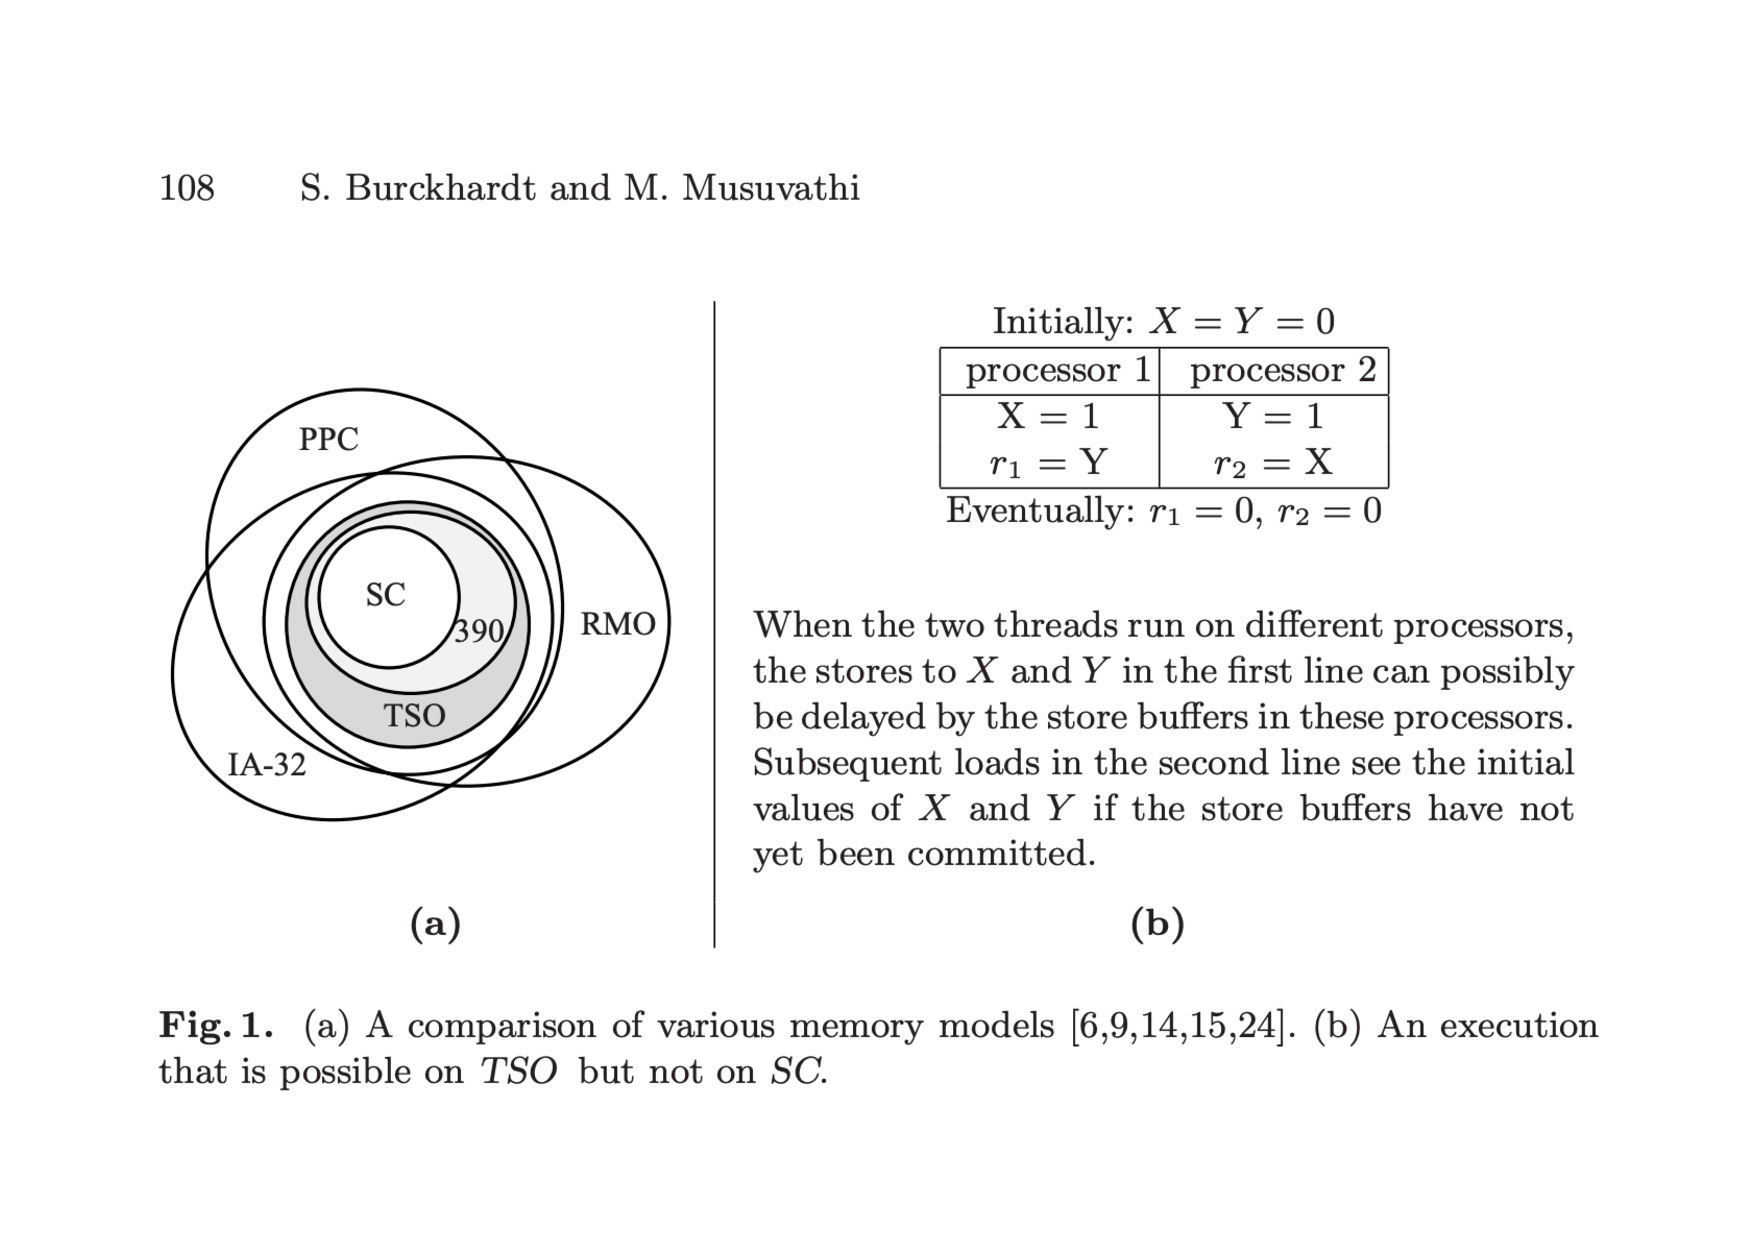
\includegraphics[width=\textwidth]{../images/MModels-and-TSO-vs-SC-BurckhardtM08.pdf}

p107:

Let $\traces_\pi^Y$ denote set of executions of program $\pi$
on memory model $Y$.

p108:

we can sensibly verify the relaxed executions
$\traces_\pi^Y$
by solving the following two verification problems separately:
\begin{enumerate}
  \item
Use standard verification methodology for concurrent programs to show that
the executions in $\traces_\pi^{SC}$ are correct.
2. Use specialized methodology for \emph{memory model safety} verification,
showing
that $\traces_\pi^Y = \traces_\pi^{SC}$ .
We say the program $\pi$ is Y-safe if $\traces_\pi^Y =\traces_\pi^{SC}$ .
\end{enumerate}

$\traces_\pi^{TSO} \subseteq \traces_\pi^Y$ for almost all models $Y$.


\subsubsection{Key Types and Sets}

p110:

\paragraph{Issue Index}
Sequence number relevant to all events by the same processor

\paragraph{Coherence Index}
sequence number of the value that is read or written by the event,
relative to the entire value sequence
written to the \emph{targeted memory location} (my emphasis) during the execution.

\begin{eqnarray*}
   o \in Op &=& \{st,ld,il\} \quad \mbox{store,load,interleave}
\\ p \in Proc &=& \{1,\dots,N\} \quad N \mbox{ fixed}
\\ a \in Adr && \mbox{finite set of addresses}
\\ i \in \Nat && \mbox{issue index}
\\ c \in \Nat_0 &=& \setof{z | z \in \Int, z \not< 0} \quad \mbox{coherence index}
\\ o(p,i,a,c), e \in Evt &=& Op \times Proc \times \Nat \times Adr \times \Nat_0
\\ o(e) &\defs& o' \mbox{ where } e = o'(p,i,a,c)
\\ p(e) &\defs& p \mbox{ where } e = o(p,i,a,c)
\\ i(e) &\defs& p \mbox{ where } e = o(p,i,a,c)
\\ a(e) &\defs& p \mbox{ where } e = o(p,i,a,c)
\\ c(e) &\defs& p \mbox{ where } e = o(p,i,a,c)
\\ E &\subseteq& Evt
\end{eqnarray*}

\begin{eqnarray*}
   E(p) &\defs& \setof{e \in E | p(e) = p}
                \quad \mbox{commands issued by processor }p
\\ L(E) &\defs& \setof{e \in E | o(e) = ld} \quad \mbox{load events }
\\ S(E) &\defs& \setof{e \in E | o(e) = st} \quad \mbox{store events }
\\ W(E) &\defs& \setof{e \in E | o(e) = \in \setof{st,il}}
                \quad \mbox{events that write}
\\ R(E) &\defs& \setof{e \in E | o(e) = \in \setof{ld,il}}
                \quad \mbox{events that read}
\\ W(E,a) &\defs& \setof{e \in W(E) | a(e) = a}
                \quad \mbox{events that write location } a
\end{eqnarray*}

\subsubsection{Traces}

Function $f:Evt \fun \Nat$ is an \emph{index} for $S' \subseteq Evt$
if $f(S') = \setof{1,\dots,|S'|}$.

\paragraph{Traces}

A trace is $E \subseteq Evt$ satisfying:
\begin{eqnarray*}
   \forall p \in Proc &\bullet& i(e) \mbox{ is an index for } E(p) \quad (E1)
\\ \forall a \in Adr &\bullet& c(e) \mbox{ is an index for } W(E,a) \quad (E2)
\\ \forall l \in L(E)
    &\bullet&
      c(l)=0
      \;\lor\;
      (\exists w \in W(E,a(l))\bullet c(l)=c(w)) \quad (E3)
\end{eqnarray*}
Let $\traces \subseteq \Set(Evt)$ be the set of all traces.

Trace $E$ is a prefix of $E'$ if $E \subseteq E'$.

p111:

\paragraph{Order Relations}

\begin{eqnarray*}
   \prgord &\subseteq& Evt \times Evt
\\ e \prgord e' &\equiv& p(e)=p(e') \land i(e) < i(e')
\\ \conflict &\subseteq& Evt \times Evt
\\ e \conflict e'
   &\equiv&
   a(e)=a(e')
   \land
\\ &&\quad (~~(o(e') \in W(Evt) \land c(e)<c(e')))
             \lor
\\ &&\qquad ((e,e')\in W(Evt)\times L(Evt)) \land c(e)\leq c(e') )
\\ \hb &\defs& (\prgord \cup \conflict)
\\ \rhb
   &\defs&
   \hb
   \setminus
   \setof{(e,e')| e \prgord e' \land o(e)=st \land o(e')=ld}
\end{eqnarray*}

\subsubsection{Memory Models}

\begin{eqnarray*}
   \traces^{SC} &\subseteq& \traces
\\ \traces^{SC} &\defs& \setof{ E | \hb \mbox{ is acyclic on } E}
\\ \traces^{TSO} &\subseteq& \traces
\\ \traces^{TSO}
   &\defs&
   \{ E | \rhb \mbox{ is acyclic on } E \quad (TSO1)
\\&& \qquad \forall e,e' \in E \bullet \lnot(e \prgord e' \land p \conflict e')
   \} \quad (TSO2)
\end{eqnarray*}
$TSO2$ guarantees that loads correctly ``snoop'' the store buffer.

\subsubsection{Program Execution}

pp111-112:

\begin{eqnarray*}
   next_\pi &:& \traces \times Proc \fun \Set(Op \times Adr)
\\ next_\pi(E,p) &\defs& \mbox{possible next instructions after } E
\\ last(E,p) &\defs& e \in E(p) |
                     i(e) \mbox{ is maximal, undefined if } E(p)=\emptyset
\end{eqnarray*}

p112:

Program $\pi$ is \emph{locally determinisitic} if
\begin{itemize}
  \item $\forall (E,p) \in \dom~ next_\pi \bullet |next_\pi(E,p)| \leq 1$
  \item $\forall E' \subseteq E
         \bullet
         last(E',p)=last(E,p)
         \implies
         next_\pi(E,p)=next_\pi(E',p)$
\end{itemize}
\textbf{It is assumed at this point that all programs are locally determinisitic}.

\begin{eqnarray*}
   succ_\pi &:& \traces \fun \Set Evt
\\ succ_\pi(E)
   &\defs&
   \{ e \in (Evt\setminus E)
      |
      (E \cup \setof e \in \traces)
      \land
      next_\pi(E,p(e))=(o(e),a(e))
   \}
\end{eqnarray*}

\paragraph{Program Traces}

\begin{eqnarray*}
   \traces_\pi^Y &\subseteq& \traces, \qquad Y \in \setof{SC,TSO}
\\ \emptyset \in \traces_\pi^Y
\\ E \cup \setof e \in \traces_\pi^Y
   &if& E \in \traces_\pi^Y
        \land e \in succ_\pi(E)
        \land E \cup \setof e \in \traces^Y
\end{eqnarray*}

\paragraph{Store Buffer Safety}

Program $\pi$ is \emph{store-buffer safe}
iff $\traces_\pi^{TSO} = \traces_\pi^{SC}$.


\subsubsection{Analysis}

\paragraph{Borderline Trace}

$E \in \traces_\pi^{SC}$ is \emph{borderline}
if $\exists e \in succ_\pi(E)
   \bullet
   E \cup \setof e \in (\traces_\pi^{TSO} \setminus \traces_\pi^{SC})$

Store-buffer safety is equivalent to having no borderline traces.

\paragraph{Cycle Characterisation}

\begin{eqnarray*}
   lastR(E,p)
   &\defs&
   e \in E(p) \cap R(e) |
       i(e) \mbox{ is maximal, or undefined if $\cap$ is empty}
\\ write(E,a,c)
   &\defs&
   e \in W(E,a) |
       c(e)=c \mbox{ if it exists, or undefined otherwise}
\end{eqnarray*}

p113:

Assume
  $E \in \traces_\pi^{SC}$;
  $e = o(p,i,a,c)$;
  and
  $E' = E \cup \setof e$:
\begin{eqnarray*}
   E' \notin \traces_\pi^{SC}
   &\equiv&
   o = ld \land write(E,a,c+1) \hb^* last(E,p)
\\ E' \notin \traces_\pi^{TSO}
   &\equiv&
   o = ld
   \land
   ( (write(E,a,c+1) \rhb^* lastR(E,p))
     \lor
     (\exists c' > c \bullet p(write(E,a,c'))=p))
\end{eqnarray*}

\newpage

p114:

Algorithm to monitor store buffer safety in a given interleaving:
\begin{verbatim}
function is_store_buffer_safe(e1e2 . . . en) returns boolean {
  var k,p,a,c : N; var E : T ;
  E := ∅;
  for (k := 1; k <= n; k++) {
    if (o(ek) = ld) {
      p := p(ek); a := a(ek); c := c(ek);
      while (c > 0) {
        if (p = i(write(E,a,c)))
          break;
        if (write(E,a,c) →∗rhb lastR(E,p))   -- need special algorithm here
          break;
        if (write(E,a,c) →∗hb last(E,p))     -- use 'vector clock' technique
          return false;
        c := c - 1;
      }
    }
    E := E ∪ ek;
  }
  return true;
}
\end{verbatim}

The above algorithm is sound for any interleaving,
and complete over a sufficient set (``representative'') of interleavings.

p116:

vector clock generalised to handle $\rhb$.

\subsubsection{Operational MM}

Also Microsoft tech report (MSR-TR-2008-12)
has some trace automata in an appendix that might be useful.

\paragraph{Trace Automata}

A \emph{trace automaton} over $Evt$ is a tuple
$$
 A = (S,T,initial,accept,guard,apply)
$$
where
\begin{itemize}
  \item $S$ is a set of states
  \item $T \supseteq Evt$ is a set of transitions,
        with $T\setminus Evt$ being considered\emph{internal}.
  \item $initial, accept : S \fun \Bool$ are self-explanatory
  \item $guard : T \fun (S \fun \Bool)$ defines the guard for each transition
  \item $apply : T \fun (S \fun S)$ defines the state-change for each transition
\end{itemize}

A sequence $\omega=\omega_0\dots\omega_n \in T^*$ is accepted by $A$
if there exists $s_0,\dots,s_{n+1} \in S$ such that:
\begin{itemize}
  \item $initial(s_0) = true$
  \item $accept(s_{n+1}) = true$
  \item $guard\seqof{w_i}(s_i) = true$
  \item $apply\seqof{w_i}(s_i) = s_{i+1}$
\end{itemize}
where $ 0 \leq i \leq n$.

\newpage
\paragraph{Sequential Consistency Automaton}

\begin{eqnarray*}
   A_{SC} &=& (S_{SC},T_{SC},initial_{SC},accept_{SC},guard_{SC},apply_{SC})
\\ T_{SC} &=& \setof{st,ld,il} \times Proc \times \Nat \times Adr \times \Nat_0
\\ S_{SC} &=& m : Adr \fun \Nat ;
              i : Proc \fun \Nat
\\ initial_{SC} &=& \forall a,p \bullet m(a)=0 \land i(p)=0
\\ accept_{SC} &=& true
\\
\\ guard_{SC}\seqof{st(p,i,a,c)} &=& i(p)=i-1 \land m(a)=c-1
\\ apply_{SC}\seqof{st(p,i,a,c)} &=& i(p):=i \land m(a):=c
\\
\\ guard_{SC}\seqof{ld(p,i,a,c)} &=& i(p)=i-1 \land m(a)=c
\\ apply_{SC}\seqof{ld(p,i,a,c)} &=& i(p):=i
\\
\\ guard_{SC}\seqof{il(p,i,a,c)} &=& i(p)=i-1 \land m(a)=c-1
\\ apply_{SC}\seqof{il(p,i,a,c)} &=& i(p):=i \land m(a):=c
\end{eqnarray*}
A state-component functions of type $I \fun V$ here
is described in the TR as \texttt{array[\textit{I}] of }$V$.
We use $f(x):=e$ as a shorthand
for function override ($f \oplus \setof{x \mapsto e}$).

\paragraph{Total Store Order Automaton}

We have a FIFO queue, here modelled as a sequence with the following operators:
\begin{eqnarray}
   q \in Q_X &=& X^*
\\ add &:& X \fun Q_X \fun Q_X
\\ add_x(q) &=& q \cat \seqof x
\\ pop &:& Q_X \fun Q_X
\\ pop(\seqof x \cat q) &:& q \quad \mbox{undefined for empty } q
\\ null &:& Q_X \fun \Bool
\\ null(q) &=& q = \seqof{}
\\ peek &:& Q_X \fun X
\\ peek(\seqof x \cat q) &=& x
\end{eqnarray}

\begin{eqnarray*}
   A_{TSO} &=& (S_{TSO},T_{TSO},initial_{TSO},accept_{TSO},guard_{TSO},apply_{TSO})
\\ T_{TSO} &=& \setof{st,st^c,ld,il} \times Proc \times \Nat \times Adr \times \Nat_0
\\ S_{TSO} &=& m : Adr \fun \Nat ;
               i : Proc \fun \Nat ;
               ml : Proc \times Adr \fun \Nat ;
               B : Proc \fun Evt^*
\\ initial_{TSO} &=& \forall a,p \bullet
                   m(a)=0 \land i(p)=0 \land ml(p,a)=0 \land null(B(p))
\\ accept_{TSO} &=& \forall p \bullet null(B(p))
\\
\\ guard_{TSO}\seqof{st(p,i,a,c)} &=& i(p)=i-1
\\ apply_{TSO}\seqof{st(p,i,a,c)}
      &=& i(p):=i \land ml(p,a):=c \land B(p):=add_{st(p,i,a,c)}(B(p))
\\
\\ guard_{TSO}\seqof{st^c(p,i,a,c)} &=& peek(B(p))=st(p,i,a,c) \land m(a)=c-1
\\ apply_{TSO}\seqof{st^c(p,i,a,c)} &=& m(a):=c \land B(p):=pop(B(p))
\\
\\ guard_{TSO}\seqof{ld(p,i,a,c)} &=& i(p)=i-1 \land c = max\setof{m(a),ml(p,a)}
\\ apply_{TSO}\seqof{ld(p,i,a,c)} &=& i(p):=i
\\
\\ guard_{TSO}\seqof{il(p,i,a,c)} &=& i(p)=i-1 \land m(a)=c-1 \land null(B(p))
\\ apply_{TSO}\seqof{il(p,i,a,c)} &=& i(p):=i \land m(a):=c
\end{eqnarray*}

\newpage\section{Atomics}\label{sec:atomics}

Here we perform an analysis of C11 Atomics to support their modelling
and consequent testing.

We will look at the following C11 atomics:
\begin{description}
  \item [Fetch-Add] \verb"obj' = atomic_fetch_add_explicit( obj, arg, order )"
  \item [Load] \verb"obj' = atomic_load_explicit( obj, order )"
  \item [Store] \verb"atomic_store_explicit( obj, desired, order )"
\end{description}
Note that the first two return a revised value for \verb"obj",
while the third has no return value.

The only memory model in scope is total-store order (TSO),
as per the SPARC architecture (sparcv8.pdf).

From \url{https://docs.oracle.com/cd/E23824_01/html/819-3196/hwovr-15.html},
we get:
\begin{quote}
``
TSO guarantees that the sequence in which store, FLUSH,
and atomic load-store instructions appear in memory for a given processor
is identical to the sequence in which they were issued by the processor.
''
\end{quote}
We note that FLUSH instructions are out-of-scope,
as their only relevance seems to be to the use of self-modifying code.

Their relevant usage is as follows:

\begin{tabular}{|c|c|}
  \hline
  Atomic Action & Memory Model(s)
\\\hline
  Load & Relaxed, Acquire
\\\hline
  Store & Relaxed, Release
\\\hline
  Fetch-Add & Relaxed
\\\hline
\end{tabular}

Given that we are working with TSO,
we find that all of the above memory models are effectively satisfied
(see
\url{https://en.cppreference.com/w/c/atomic/memory_order#Release-Acquire_ordering}
).

\subsection{Atomic Load Explicit}

Given atomic object type \texttt{A} and value type \texttt{C}:
\begin{nicec}
C atomic_load_explicit( const volatile A* obj, memory_order order )
\end{nicec}
then, with TSO, and \texttt{order} being relaxed, acquire or release,
we have:
\begin{nicec}
result = atomic_load_explicit( obj, order );
\end{nicec}
is equivalent to:
\begin{nicec}
atomic{ result = *obj  }
\end{nicec}

Usage:
\begin{nicec}
_Atomic_Load_uint( &gate->go_ahead, ATOMIC_ORDER_RELAXED )
_Atomic_Load_uint( &lock->now_serving, ATOMIC_ORDER_ACQUIRE )
_Atomic_Load_uint( &lock->now_serving, ATOMIC_ORDER_RELAXED )
_Atomic_Load_uint( &the_thread->Wait.flags, ATOMIC_ORDER_RELAXED )
_Atomic_Load_uint( &the_thread->Wait.flags, ATOMIC_ORDER_ACQUIRE )
\end{nicec}


\subsection{Store Load Explicit}

Given atomic object type \texttt{A} and value type \texttt{C}:
\begin{nicec}
void atomic_store_explicit( volatile A* obj, C desired, memory_order order )
\end{nicec}
then, with TSO, and \texttt{order} being relaxed, acquire or release,
we have:
\begin{nicec}
atomic_store_explicit( obj, desired, order );
\end{nicec}
is equivalent to:
\begin{nicec}
atomic{ *obj = desired }
\end{nicec}

Usage:
\begin{nicec}
_Atomic_Store_uint( &gate->go_ahead, 0, ATOMIC_ORDER_RELAXED )
_Atomic_Store_uint( &gate->go_ahead, 1, ATOMIC_ORDER_RELAXED )
_Atomic_Store_uint( &lock->now_serving, next_ticket, ATOMIC_ORDER_RELEASE )
_Atomic_Store_uint( &the_thread->Wait.flags, flags, ATOMIC_ORDER_RELAXED )
\end{nicec}

\subsection{Atomic Fetch-Add}

Given atomic object type \texttt{A}, value \texttt{C},
and value or pointer-difference type \texttt{M}:
\begin{nicec}
C atomic_fetch_add_explicit( volatile A* obj, M arg, memory_order order )
\end{nicec}
then, with TSO, and \texttt{order} being relaxed, acquire or release,
we have:
\begin{nicec}
result = atomic_fetch_add_explicit( obj, arg, order )
\end{nicec}
is equivalent to:
\begin{nicec}
atomic{ result = *obj ; *obj = *obj + arg }
\end{nicec}

Usage:
\begin{nicec}
_Atomic_Fetch_add_uint( &lock->next_ticket, 1U, ATOMIC_ORDER_RELAXED )
\end{nicec}

\newpage\section{Code Notes}

Wanted: call sequence paths from
\verb"rtems_semaphore_obtain()"
and
\verb"rtems_semaphore_release()",
via
\verb"_Thread_queue_Enqueue()"
and
\verb"_Thread_queue_Surrender()"
to
\verb"_Thread_Wait_acquire_critical".

The routing may also involve:
\verb"_Thread_queue_Gate_add",
\verb"_Thread_queue_Gate_wait",
and
\verb"_Thread_queue_Gate_open".

\subsection{Creating a Semaphore}

This is setup by a call to \verb"rtems_semaphore_create"
with options for
\begin{description}
  \item [queue discipline] \verb"RTEMS_PRIORITY"
  \item [semaphore class] \verb"RTEMS_BINARY_SEMAPHORE"
  \item [locking protocol] \verb"RTEMS_INHERIT_PRIORITY"
\end{description}
There is a \verb"SEMAPHORE_KIND_MASK"
that contains \verb"RTEMS_INHERIT_PRIORITY".
\begin{nicec}
attr = RTEMS_BINARY_SEMAPHORE |  RTEMS_PRIORITY | RTEMS_INHERIT_PRIORITY ;
rc = rtems_semaphore_create( "SEMA", 1, attr, _ &semId );
\end{nicec}
Internally:
\begin{nicec}
#define RTEMS_SEMAPHORE_CLASS 0x00000030 // (incl. RTEMS_BINARY_SEMAPHORE )
#define SEMAPHORE_KIND_MASK ( RTEMS_SEMAPHORE_CLASS | RTEMS_INHERIT_PRIORITY \
  | RTEMS_PRIORITY_CEILING | RTEMS_MULTIPROCESSOR_RESOURCE_SHARING )

  maybe_global = RTEMS_INHERIT_PRIORITY; // attribute_set & SEMAPHORE_KIND_MASK
  mutex_with_protocol =  attr ;
    // attribute_set & ( SEMAPHORE_KIND_MASK | RTEMS_GLOBAL | RTEMS_PRIORITY )

  } else if (
    mutex_with_protocol
      == ( RTEMS_BINARY_SEMAPHORE | RTEMS_PRIORITY | RTEMS_INHERIT_PRIORITY )
  ) {
    variant = SEMAPHORE_VARIANT_MUTEX_INHERIT_PRIORITY;  // ... }

  the_semaphore = _Semaphore_Allocate();
  // include/rtems/rtems/semimpl.h
  flags = SEMAPHORE_VARIANT_MUTEX_INHERIT_PRIORITY;
         // _Semaphore_Set_variant( 0, variant );
  if ( _Attributes_Is_priority( attribute_set ) ) {
    flags = _Semaphore_Set_discipline( flags, SEMAPHORE_DISCIPLINE_PRIORITY );
  _Semaphore_Set_flags( the_semaphore, flags );
  executing = _Thread_Get_executing();
  switch ( variant ) {
    case SEMAPHORE_VARIANT_MUTEX_INHERIT_PRIORITY:
      _CORE_recursive_mutex_Initialize(
        &the_semaphore->Core_control.Mutex.Recursive
      );
      if ( count == 0 ) {
        _CORE_mutex_Set_owner(
          &the_semaphore->Core_control.Mutex.Recursive.Mutex,
          executing
        );
        _Thread_Resource_count_increment( executing );
      }
      status = STATUS_SUCCESSFUL;
      break;
  }
  _Objects_Open(
    &_Semaphore_Information,
    &the_semaphore->Object,
    (Objects_Name) name
  );
  *id = the_semaphore->Object.id;
  _Objects_Allocator_unlock();
  return RTEMS_SUCCESSFUL;
}
\end{nicec}

So
 variable \verb"maybe_global" will contain \verb"RTEMS_INHERIT_PRIORITY",
 and \verb"mutex_with_protocol" will contain \verb"RTEMS_PRIORITY".

 Given these, then we set \verb"variant"
 to \verb"SEMAPHORE_VARIANT_MUTEX_INHERIT_PRIORITY".


From \texttt{coremuteximpl.h}:
\begin{nicec}
// 49:
RTEMS_INLINE_ROUTINE void _CORE_mutex_Initialize(
  CORE_mutex_Control *the_mutex
)
{
  _Thread_queue_Object_initialize( &the_mutex->Wait_queue );
}

// 182:
RTEMS_INLINE_ROUTINE void _CORE_recursive_mutex_Initialize(
  CORE_recursive_mutex_Control *the_mutex
)
{
  _CORE_mutex_Initialize( &the_mutex->Mutex );
  the_mutex->nest_level = 0;
}
\end{nicec}

From: \texttt{threadq.c}:
\begin{nicec}
// 144:
void _Thread_queue_Initialize(
  Thread_queue_Control *the_thread_queue,
  const char           *name
)
{
  _Thread_queue_Queue_initialize( &the_thread_queue->Queue, name );
#if defined(RTEMS_SMP)
  _SMP_lock_Stats_initialize( &the_thread_queue->Lock_stats, "Thread Queue" );
#endif
}
// 155:
void _Thread_queue_Object_initialize( Thread_queue_Control *the_thread_queue )
{
  _Thread_queue_Initialize( the_thread_queue, _Thread_queue_Object_name );
}
\end{nicec}

From \texttt{threadqimpl.h}:
\begin{nicec}
// 545:
RTEMS_INLINE_ROUTINE void _Thread_queue_Queue_initialize(
  Thread_queue_Queue *queue,
  const char         *name
)
{
#if defined(RTEMS_SMP)
  _SMP_ticket_lock_Initialize( &queue->Lock );
#endif
  queue->heads = NULL;
  queue->owner = NULL;
  queue->name = name;
}
\end{nicec}

\subsection{Obtaining a Semaphore}

We assume a binary, priority inherit semaphore,
as created above.

We consider a call to obtain a semaphore that will wait (forever)
\begin{nicec}
rc = rtems_semaphore_obtain( semId, RTEMS_WAIT, RTEMS_NO_TIMEOUT );
\end{nicec}
Internally:
\begin{nicec}
  the_semaphore = _Semaphore_Get( semId, &queue_context );
  executing = _Thread_Executing;
  // cpukit/include/rtems/rtems/optionsimpl.h
  wait = true; // !_Options_Is_no_wait( RTEMS_WAIT );
  if ( wait ) {
    // _Thread_queue_Context_set_enqueue_timeout_ticks( &queue_context, timeout );
    queue_context->Timeout.ticks = ticks;
    queue_context->enqueue_callout = _Thread_queue_Add_timeout_ticks;

  flags = _Semaphore_Get_flags( the_semaphore );
  variant = SEMAPHORE_VARIANT_MUTEX_INHERIT_PRIORITY
            // _Semaphore_Get_variant( flags );

  switch ( variant ) {
    case SEMAPHORE_VARIANT_MUTEX_INHERIT_PRIORITY:
      status = _CORE_recursive_mutex_Seize(
        &the_semaphore->Core_control.Mutex.Recursive,
        CORE_MUTEX_TQ_PRIORITY_INHERIT_OPERATIONS,
        executing,
        wait,
        _CORE_recursive_mutex_Seize_nested,
        &queue_context
      );
      break;
  }
  return _Status_Get( status );
\end{nicec}

Now, seizing that mutex:
\begin{nicec}
/**
 * @brief Seizes the recursive mutex.
 *
 * @param[in, out] the_mutex The recursive mutex to seize.
 * @param operations The thread queue operations.
 * @param[out] executing The executing thread.
 * @param wait Indicates whether the calling thread is willing to wait.
 * @param nested Returns the status of a recursive mutex.
 * @param queue_context The thread queue context.
 *
 * @retval STATUS_SUCCESSFUL The owner of the mutex was NULL, successful
 *      seizing of the mutex.
 * @retval _Thread_Wait_get_status The status of the executing thread.
 * @retval STATUS_UNAVAILABLE The calling thread is not willing to wait.
 */
RTEMS_INLINE_ROUTINE Status_Control _CORE_recursive_mutex_Seize(
  CORE_recursive_mutex_Control  *the_mutex,
  const Thread_queue_Operations *operations,
  Thread_Control                *executing,
  bool                           wait,
  Status_Control              ( *nested )( CORE_recursive_mutex_Control * ),
  Thread_queue_Context          *queue_context
)
{
  Thread_Control *owner;

  _CORE_mutex_Acquire_critical( &the_mutex->Mutex, queue_context );

  owner = _CORE_mutex_Get_owner( &the_mutex->Mutex );

  if ( owner == NULL ) {
    _CORE_mutex_Set_owner( &the_mutex->Mutex, executing );
    _Thread_Resource_count_increment( executing );
    _CORE_mutex_Release( &the_mutex->Mutex, queue_context );
    return STATUS_SUCCESSFUL;
  }

  if ( owner == executing ) {
    Status_Control status;

    status = ( *nested )( the_mutex );
    _CORE_mutex_Release( &the_mutex->Mutex, queue_context );
    return status;
  }

  return _CORE_mutex_Seize_slow(
    &the_mutex->Mutex,
    operations,
    executing,
    wait,
    queue_context
  );
}
\end{nicec}


\coremutexseizeC:
\begin{nicec}
Status_Control _CORE_mutex_Seize_slow(
  CORE_mutex_Control            *the_mutex,
  const Thread_queue_Operations *operations,
  Thread_Control                *executing,
  bool                           wait,
  Thread_queue_Context          *queue_context
)
{
  if ( wait ) {
    _Thread_queue_Context_set_thread_state(
      queue_context,
      STATES_WAITING_FOR_MUTEX
    );
    _Thread_queue_Context_set_deadlock_callout(
      queue_context,
      _Thread_queue_Deadlock_status
    );
    _Thread_queue_Enqueue(
      &the_mutex->Wait_queue.Queue,
      operations,
      executing,
      queue_context
    );
    return _Thread_Wait_get_status( executing );
  } else {
    _CORE_mutex_Release( the_mutex, queue_context );
    return STATUS_UNAVAILABLE;
  }
}
\end{nicec}

\threadqenqueueC:
\begin{nicec}
void _Thread_queue_Enqueue(
  Thread_queue_Queue            *queue,
  const Thread_queue_Operations *operations,
  Thread_Control                *the_thread,
  Thread_queue_Context          *queue_context
)
{
  Per_CPU_Control *cpu_self;
  bool             success;

  _Assert( queue_context->enqueue_callout != NULL );

  _Thread_Wait_claim( the_thread, queue );

  if ( !_Thread_queue_Path_acquire_critical( queue, the_thread, queue_context ) ) {
    _Thread_queue_Path_release_critical( queue_context );
    _Thread_Wait_restore_default( the_thread );
    _Thread_queue_Queue_release( queue, &queue_context->Lock_context.Lock_context );
    _Thread_Wait_tranquilize( the_thread );
    _Assert( queue_context->deadlock_callout != NULL );
    ( *queue_context->deadlock_callout )( the_thread );
    return;
  }

  _Thread_queue_Context_clear_priority_updates( queue_context );
  _Thread_Wait_claim_finalize( the_thread, operations );
  ( *operations->enqueue )( queue, the_thread, queue_context );

  _Thread_queue_Path_release_critical( queue_context );

  the_thread->Wait.return_code = STATUS_SUCCESSFUL;
  _Thread_Wait_flags_set( the_thread, THREAD_QUEUE_INTEND_TO_BLOCK );
  cpu_self = _Thread_queue_Dispatch_disable( queue_context );
  _Thread_queue_Queue_release( queue, &queue_context->Lock_context.Lock_context );

  ( *queue_context->enqueue_callout )(
    queue,
    the_thread,
    cpu_self,
    queue_context
  );

  /*
   *  Set the blocking state for this thread queue in the thread.
   */
  _Thread_Set_state( the_thread, queue_context->thread_state );

  /*
   * At this point thread dispatching is disabled, however, we already released
   * the thread queue lock.  Thus, interrupts or threads on other processors
   * may already changed our state with respect to the thread queue object.
   * The request could be satisfied or timed out.  This situation is indicated
   * by the thread wait flags.  Other parties must not modify our thread state
   * as long as we are in the THREAD_QUEUE_INTEND_TO_BLOCK thread wait state,
   * thus we have to cancel the blocking operation ourself if necessary.
   */
  success = _Thread_Wait_flags_try_change_acquire(
    the_thread,
    THREAD_QUEUE_INTEND_TO_BLOCK,
    THREAD_QUEUE_BLOCKED
  );
  if ( !success ) {
    _Thread_Remove_timer_and_unblock( the_thread, queue );
  }

  _Thread_Priority_update( queue_context );
  _Thread_Dispatch_direct( cpu_self );
}
\end{nicec}
The loop whose termination  is an issue can be found in
\verb"_Thread_queue_Path_acquire_critical",
also in the same file.

\begin{nicec}
#if !defined(RTEMS_SMP)
static
#endif
bool _Thread_queue_Path_acquire_critical(
  Thread_queue_Queue   *queue,
  Thread_Control       *the_thread,
  Thread_queue_Context *queue_context
)
{
  Thread_Control     *owner;
#if defined(RTEMS_SMP)
  Thread_queue_Link  *link;
  Thread_queue_Queue *target;

  /*
   * For an overview please look at the non-SMP part below.  We basically do
   * the same on SMP configurations.  The fact that we may have more than one
   * executing thread and each thread queue has its own SMP lock makes the task
   * a bit more difficult.  We have to avoid deadlocks at SMP lock level, since
   * this would result in an unrecoverable deadlock of the overall system.
   */

  _Chain_Initialize_empty( &queue_context->Path.Links );

  owner = queue->owner;

  if ( owner == NULL ) {
    return true;
  }

  if ( owner == the_thread ) {
    return false;
  }

  _Chain_Initialize_node(
    &queue_context->Path.Start.Lock_context.Wait.Gate.Node
  );
  link = &queue_context->Path.Start;
  _RBTree_Initialize_node( &link->Registry_node );
  _Chain_Initialize_node( &link->Path_node );

  do {
    _Chain_Append_unprotected( &queue_context->Path.Links, &link->Path_node );
    link->owner = owner;

    _Thread_Wait_acquire_default_critical(
      owner,
      &link->Lock_context.Lock_context
    );

    target = owner->Wait.queue;
    link->Lock_context.Wait.queue = target;

    if ( target != NULL ) {
      if ( _Thread_queue_Link_add( link, queue, target ) ) {
        _Thread_queue_Gate_add(
          &owner->Wait.Lock.Pending_requests,
          &link->Lock_context.Wait.Gate
        );
        _Thread_Wait_release_default_critical(
          owner,
          &link->Lock_context.Lock_context
        );
        _Thread_Wait_acquire_queue_critical( target, &link->Lock_context );

        if ( link->Lock_context.Wait.queue == NULL ) {
          _Thread_queue_Link_remove( link );
          _Thread_Wait_release_queue_critical( target, &link->Lock_context );
          _Thread_Wait_acquire_default_critical(
            owner,
            &link->Lock_context.Lock_context
          );
          _Thread_Wait_remove_request_locked( owner, &link->Lock_context );
          _Assert( owner->Wait.queue == NULL );
          return true;
        }
      } else {
        link->Lock_context.Wait.queue = NULL;
        _Thread_queue_Path_append_deadlock_thread( owner, queue_context );
        return false;
      }
    } else {
      return true;
    }

    link = &owner->Wait.Link;
    queue = target;
    owner = queue->owner;
  } while ( owner != NULL );
#else
  do {
    owner = queue->owner;

    if ( owner == NULL ) {
      return true;
    }

    if ( owner == the_thread ) {
      return false;
    }

    queue = owner->Wait.queue;
  } while ( queue != NULL );
#endif

  return true;
}  
\end{nicec}


\subsection{Lower down\dots}

The code mentioned by Sebastian, from \threadimplH:
\begin{nicec}
/**
 * @brief Acquires the thread wait lock inside a critical section (interrupts
 * disabled).
 *
 * @param[in, out] the_thread The thread.
 * @param[in, out] queue_context The thread queue context for the corresponding
 *   _Thread_Wait_release_critical().
 */
RTEMS_INLINE_ROUTINE void _Thread_Wait_acquire_critical(
  Thread_Control       *the_thread,
  Thread_queue_Context *queue_context
)
{
#if defined(RTEMS_SMP)
  Thread_queue_Queue *queue;

  _Thread_Wait_acquire_default_critical(
    the_thread,
    &queue_context->Lock_context.Lock_context
  );

  queue = the_thread->Wait.queue;
  queue_context->Lock_context.Wait.queue = queue;

  if ( queue != NULL ) {
    _Thread_queue_Gate_add(
      &the_thread->Wait.Lock.Pending_requests,
      &queue_context->Lock_context.Wait.Gate
    );
    _Thread_Wait_release_default_critical(
      the_thread,
      &queue_context->Lock_context.Lock_context
    );
    _Thread_Wait_acquire_queue_critical( queue, &queue_context->Lock_context );

    if ( queue_context->Lock_context.Wait.queue == NULL ) {
      _Thread_Wait_release_queue_critical(
        queue,
        &queue_context->Lock_context
      );
      _Thread_Wait_acquire_default_critical(
        the_thread,
        &queue_context->Lock_context.Lock_context
      );
      _Thread_Wait_remove_request_locked(
        the_thread,
        &queue_context->Lock_context
      );
      _Assert( the_thread->Wait.queue == NULL );
    }
  }
#else
  (void) the_thread;
  (void) queue_context;
#endif
}

\end{nicec}

\newpage\subsection{Code Index}

All paths are relative to \texttt{rtems/cpukit}.


\def\ditto{~~~~~''}

\begin{tabular}{lr@{ : }l}
   \verb"go_ahead" &  120 & \threadqH
\\ \ditto          &  470 & \threadqimplH
\\ \ditto          &  496 & \threadqimplH
\\ \ditto          &  510 & \threadqimplH
\\ \verb"rtems_semaphore_create"            &  218 & \semH
\\ \ditto                                   &   35 & \semcreateH
\\ \verb"rtems_semaphore_obtain"            &   53 & \semobtainC
\\ \verb"rtems_semaphore_release"           &   26 & \semreleaseC
\\ \verb"_Thread_queue_Enqueue"             &  387 & \threadqenqueueC
\\ \verb"_Thread_queue_Surrender"           &  667 & \threadqenqueueC
\\ \verb"_Thread_Wait_acquire_critical"     & 1795 & \threadimplH
\\ \verb"_Thread_Add_timeout_ticks"         & 2388 & \threadimplH
\\ \verb"_Thread_queue_Gate_add"            &  479 & \threadqimplH
\\ \verb"_Thread_queue_Gate_wait"           &  506 & \threadqimplH
\\ \verb"_Thread_queue_Gate_open"           &  492 & \threadqimplH
\\ \verb"_Thread_queue_Do_acquire_critical" &  663 & \threadqimplH
\\ \verb"_Thread_queue_Acquire_critical"    &  679 & \threadqimplH
\\ \verb"_Thread_Resource_count_increment"  & 1322 & \threadimplH
\\ \verb"Thread_queue_Gate"                 &  121 & \threadqH
\\ \verb"THREAD_QUEUE_OBJECT_ASSERT"        & 1452 & \threadqimplH
\\ \verb"RTEMS_STATIC_ASSERT"               &  759 & \basedefsH
\\ \verb"_CORE_recursive_mutex_Initialize"  &  182 & \coremuteximplH
\\ \verb"_CORE_recursive_mutex_Seize"       &  220 & \coremuteximplH
\\ \verb"_CORE_mutex_Acquire_critical"      &   72 & \coremuteximplH
\\ \verb"_CORE_mutex_Get_owner"             &  101 & \coremuteximplH
\\ \verb"_CORE_mutex_Set_owner"             &  152 & \coremuteximplH
\\ \verb"_Thread_queue_Add_timeout_ticks"   &   28 & \threadqtimeoutC
\\ \verb"_CORE_mutex_Release"               &   86 & \coremutexseizeC
\\ \verb"_CORE_mutex_Seize_slow"            &  138 & \coremuteximplH
\\ \ditto                                   &   28 & \coremutexseizeC
\\ \verb"_Thread_queue_Context_set_thread_state" &  176 & \threadqimplH
\\ \verb" _Thread_queue_Context_set_deadlock_callout" &  322 & \threadqimplH
\\ \verb"_Thread_queue_Enqueue" &  387 & \threadqenqueueC
\\ \verb"_Thread_Wait_get_status" & 2337 & \threadimplH
\end{tabular}


\newpage\section{Thread Q Req-Spec}

Here we assemble notes about thread-Q requirements and specifications,
at a high level of abstraction.

A key concern is the maintenance of FIFO fairness.

\subsection{Scope}

We are working with scenarios involving semaphores
setup to be binary, using the priority inheritance protocol.

This requires the following semaphore attributes:
\begin{verbatim}
RTEMS_PRIORITY
RTEMS_BINARY_SEMAPHORE
RTEMS_INHERIT_PRIORITY
RTEMS_MULTIPROCESSOR_RESOURCE_SHARING
\end{verbatim}

This means we are using the MrsP protocol.

All notes below assume the above setup.

\subsection{Semaphore calls}

``
Call \verb"semaphore_obtain()" can return \verb"RTEMS_UNSATISFIED"
if there is a deadlock detected,
or it has been recursively called  by the same task.''

``Call \verb"semaphore_release()" can return \verb"RTEMS_INCORRECT_STATE"
if the calling task did did not respect
the expected acquisition and  release order.
Semaphores using this protocol must be released
in the opposite order with respect to the order in which they were obtained.''


MrsP requires a pre-scheduler ceiling priority for every mutex.
This is set using the \verb"priority_ceiling"  argument
of \verb"rtems_semaphore_create".

The above is from:
Bloom, Gedare; Sherrill, Joel; Hu, Tingting; Bertolotti, Ivan Cibrario.
Real-Time Systems Development with RTEMS and Multicore Processors
(Embedded Systems) (p. 245). CRC Press. Kindle Edition.

Bloom, G., Sherrill, J., Hu, T., \& Bertolotti, I.C. (2020).
Real-Time Systems Development with RTEMS and Multicore Processors (1st ed.).
CRC Press.
\verb"https://doi.org/10.1201/9781351255790"

\subsection{Priority Inheritance Protocol (PIP)}

``
The general idea of the priority inheritance protocol is to
dynamically increase the priority of a task
as soon as it is blocking some higher-priority tasks,
and run the  task at increased priority until it is no longer blocking them.
For example, as long as  a task (like $\tau$3 in Figure 8.1)
is blocking a higher-priority task (like $\tau$1 in the same  fgure)
it inherits its priority.''

``
In general,
as long as a task is blocking a set of higher-priority tasks,
it inherits the highest priority among them.''

Bloom, Gedare; Sherrill, Joel; Hu, Tingting; Bertolotti, Ivan Cibrario. Real-Time Systems Development with RTEMS and Multicore Processors (Embedded Systems) (p. 283). CRC Press. Kindle Edition.

We have:
\begin{itemize}
  \item task baseline vs. active priority
  \item scheduler uses active priority, with FCFS for same priority
  \item semaphore wait queues ordered by active priority.
\end{itemize}

\subsection{Priority Ceiling Protocol (PCP)}

This is PIP with the following added:
``
a task can be blocked not only because it attempted to acquire a busy semaphore,
as it happens for all kinds of mutual exclusion semaphore,
but also when acquiring a free semaphore could lead
a higher-priority task to be blocked more than once.''

Bloom, Gedare; Sherrill, Joel; Hu, Tingting; Bertolotti, Ivan Cibrario. Real-Time Systems Development with RTEMS and Multicore Processors (Embedded Systems) (p. 287). CRC Press. Kindle Edition.

We have that:
\begin{itemize}
  \item each semaphore has a fixed ceiling value,
  equal to the maximum initial priority of all tasks using the semaphore.
\end{itemize}

``
\begin{enumerate}
  \item
    When a task $\tau$ tries to acquire a semaphore,
    its active priority is checked against
    the ceiling of all currently busy semaphores,
    except the ones that $\tau$ has already acquired in the past and not released yet.
  \item
    If the active priority of $\tau$ is higher than all those ceilings,
    $\tau$ can proceed with the semaphore operation
    and possibly block if the semaphore is busy.
  \item
    Otherwise, $\tau$ is blocked until this condition becomes true,
    regardless of whether  the semaphore it is trying to acquire is busy or free.
    Afterwards, $\tau$ can proceed  with the semaphore operation.
\end{enumerate}
''

Bloom, Gedare; Sherrill, Joel; Hu, Tingting; Bertolotti, Ivan Cibrario. Real-Time Systems Development with RTEMS and Multicore Processors (Embedded Systems) (p. 288). CRC Press. Kindle Edition.

\subsection{Immediate Priority Ceiling Protocol (IPCP)}%
\footnote{
a.k.a. Priority Ceiling Emulation Protocol (PCEP)
}

Like IPCP, except that when a task acquires a semaphore its active priority
is immediately raised to the semaphore ceiling.

``
More formally,
at each instant
the active priority of a task is equal to the maximum
among its baseline priority
and the ceilings of all semaphores it has acquired and not released  yet so far.''

Bloom, Gedare; Sherrill, Joel; Hu, Tingting; Bertolotti, Ivan Cibrario. Real-Time Systems Development with RTEMS and Multicore Processors (Embedded Systems) (p. 288). CRC Press. Kindle Edition.

\textbf{Note: }
\textsf{Any change in task priority means updating the relevant queues}.

\subsection{Multiprocessor Resource Sharing Protocol (MrsP)}

This is derived from the priority ceiling protocols above.

``MrsP requires programmers to specify,
for each semaphore,
what is the priority of the highest-priority task
that can ever acquire that semaphore,
for each scheduler instance.
As a result,
each MrsP semaphore has multiple priority ceiling values,
one for each scheduler instance in the system.''

Bloom, Gedare; Sherrill, Joel; Hu, Tingting; Bertolotti, Ivan Cibrario. Real-Time Systems Development with RTEMS and Multicore Processors (Embedded Systems) (p. 456). CRC Press. Kindle Edition.

We note that:
\begin{itemize}
  \item
    ``When a task successfully acquires a semaphore,
      its priority is temporarily elevated
      to the ceiling priority of the semaphore
      for the scheduler instance the task is normally assigned to.
      In RTEMS,
      this scheduler instance is also called
      the home scheduler instance of the task.
      The priority elevation lasts until the task releases the semaphore.
      From this point of view,
      MrsP works in the same way as the immediate priority ceiling  protocol.''
  \item
    ``Tasks that are waiting to acquire a semaphore spin,
      that is,
      perform an active wait
      and remain running from the scheduler’s point of view,
      instead of waiting passively by
      moving to the blocked state of the task state diagram.
      Informally speaking,
      this prevents the spinning task from
      suffering further priority inversion-induced blocking
      after it eventually acquires the  semaphore,
      due to lower-priority tasks that might have been run
      and have  had their priority elevated by MrsP in the meantime.''
  \item
    ``In some cases,
      a helping protocol among scheduler instances
      may temporarily migrate a task from
      the set of cores it is normally assigned to,
      according to the partitioned or clustered scheduling approach,
      onto other cores.
      In the most basic case,
      this happens when the task is preempted
      by a higher priority task while it holds a semaphore,
      and on the other core there is a task waiting for the same semaphore.
      In other words,
      this also means that a task  may temporarily execute
      on cores that are not managed by its own home  scheduler instance,
      but belong to other scheduler instances
      where there is  at least another task that shares a semaphore with it.''
\end{itemize}

Bloom, Gedare; Sherrill, Joel; Hu, Tingting; Bertolotti, Ivan Cibrario. Real-Time Systems Development with RTEMS and Multicore Processors (Embedded Systems) (p. 457). CRC Press. Kindle Edition. ''

\subsection{MrsP on RTEMS}

A MrsP semaphore is built unlocked, with a given ceiling priority.
It's ceiling priority w.r.t. some scheduler may be different
and so may need tailoring.

Restrictions:
\begin{itemize}
  \item
    ``Tasks must release MrsP semaphores in the reverse order
      with respect to the sequence in which they were acquired,
      as it comes natural if critical regions are properly nested.
      Attempts to deviate from the prescribed order
      are detected and reported with
      the \verb"RTEMS_INCORRECT_STATE" status code upon semaphore release.''
  \item
    ``MrsP semaphores cannot be acquired recursively.
    Any attempt to do so results in
    the \verb"RTEMS_UNSATISFIED" status code being returned
    by \verb"rtems_semaphore_obtain".''
  \item
    ``Besides self-deadlocks
      that would result from recursive semaphore acquisition,
      the system also detects more complex kinds of deadlock
      that would be created by acquiring a semaphore.
      In this case, the \verb"rtems_semaphore_obtain" directive fails
      and returns the status code  \verb"RTEMS_UNSATISFIED".''
  \item
    ``Finally,
      but this is a restriction that does not concern only MrsP semaphores,
      an MrsP semaphore cannot be taken from an interrupt context
      or whenever thread dispatching is disabled.
      Any attempt to do so results in an internal RTEMS error
      or undefined behavior.''
\end{itemize}

Bloom, Gedare; Sherrill, Joel; Hu, Tingting; Bertolotti, Ivan Cibrario. Real-Time Systems Development with RTEMS and Multicore Processors (Embedded Systems) (p. 458). CRC Press. Kindle Edition. ''


\subsection{The MrsP Paper}

Notation: $\textrm{Quantity}_{\textrm{task}}^{\textrm{resource}}$.

Worst time execution of any task using resource $j$ is $c^j$.

No. of processors with tasks that access $r^j$ is $|map(G(r^j))|$.
$$
e_j = |map(G(r^j))|c^j
$$

\begin{quote}
``
Under MrsP we incorporate the property,
fundamental to the PCP/SRP protocol,
that once a task starts executing,
its resources will be logically available
–--
but the execution time required to use the resource is $e^j$ , not $c^j$ .
''
\end{quote}

From Section VI of MrsP paper (Burns and Wellings):


\begin{enumerate}
  \item
    All resources are assigned a set of ceiling priorities,
    one per processor
    (for those processors that have tasks that use the resource);
    for processor $p_k$ it is the maximum priority
    of all tasks allocated to $p_k$ that use the resource.
  \item
    An access request on any resource results
    in the priority of the task
    being immediately raised to the local ceiling for the resource.
  \item
    Accesses to a resource are dealt with in a FIFO order.
  \item
    While waiting to gain access to the resource,
    and while actually using the resource,
    the task continues to be active and executes
    (possible spinning)
    with priority equal to the local ceiling of the resource.
  \item
    Any task waiting to gain access to a resource
    must be capable of undertaking the associated computation
    on behalf of any other waiting task.
  \item
    This cooperating task must undertake
    the outstanding requests in the original FIFO order.
\end{enumerate}

\begin{quote}
``
The setting of the local ceiling for the resource
and the raising of the accessing task’s priority to the ceiling level
means that each processor implements a local PCP/SRP protocol.
''
\end{quote}

\begin{quote}
``
The key notion here is that a task is not spinning uselessly
while it is waiting to access the resource,
rather it is prepared to use its ‘wasted cycles’
to help other tasks make progress.
''
\end{quote}

\subsubsection{MrsP Properties}

\begin{description}
  \item [Lemma 1]
    ``
    At most one task per processor can be attempting
    to access any specific resource.
    ''
  \item [Lemma 2]
    ``
    The maximum length of the FIFO queue for resource $r^k$
    is $|map(G(r^k))|$.
    ''
  \item [Lemma 3]
    ``
    Each job can suffer at most a single local block,
    and this blocking will occur before it actually executes.
    ''
\end{description}

\subsubsection{Realising MrsP}

Task Migration:

\begin{quote}
``
If a task, $\tau_a$, is preempted whilst accessing a resource, $r^i$,
(by a higher priority local task)
then $\tau_a$ can migrate to any processor
on which a task is spinning
waiting to gain access to the same resource.
On this new processor $\tau_a$ is given the priority
one higher than the spinning task so that it preempts the spinning task.
''
\end{quote}

\begin{quote}
``
\dots
the requirement of the protocol:
that any spinning task can take over the resource access
on behalf of any other task is satisfied.
The spinning task just gives way to the migrating task
as the new task has a slightly higher priority.
In practice,
the supporting RTOS must be aware
that there is a separate priority associated
with each processor in the thread’s affinity set.
''
\end{quote}

\subsubsection{Prototype Implementation of MrsP}

Task t on processor p wants a lock on resource R:
\begin{verbatim}
Lock (R, t, p) ->
  raise priority of t to local ceiling of R
  Affinities(R) := Affinities(R) + p
  if already locked
    get current resource user R(t)
    Affinities(R(t)) := Affinities(R)
    obtain FIFO lock on R and spin
  else
    Affinities(t) := Affinities(R)
  end if
  set current lock holder to self
  raise priority of t by 1
  -- use R
\end{verbatim}

Releasing the lock on R held by task t, originally on processor p:
\begin{verbatim}
Unlock(R, t, p) ->
  Affinities(R) := Affinities(R) - p
  Release next task in FIFO queue (if there is one)
  Affinities(t) := p
  lower priority of t to its base value
\end{verbatim}


\subsection{The MrsP in RTEMS Thesis}

From:
Gomes. Ricardo,
``Analysis of MrsP Protocol in RTEMS Operating System'',
Licenciatura thesis,
Departmento de Engenharia Inform\'{a}tica, CISTER, Porto,
2019.

\begin{quotation}
``
In order to support the helping mechanism,
the RTEMS scheduler needs three indispensable operations,
“ask a scheduler node for help”,
“reconsider the help request of a scheduler node”
and “withdraw a scheduler node”
'' (pp34--35)
\end{quotation}

\begin{quotation}
``
MrsP is considered a mutex,
or binary semaphore,
since only one task at a time may obtain it,
granting mutual exclusion of resources.
Thus, being considered a resource sharing protocol.
Tasks access order to MrsP semaphores are dealt according to their priorities.
'' (p39)
\end{quotation}

\begin{quotation}
``
In this chapter,
the focus is the implementation of the most relevant operations
of a MrsP semaphore in RTEMS,
namely,
the creation of a semaphore,
changing its priority ceiling,
the resource release,
resource obtainment and,
finally,
the semaphore deletion.
`` (p41)
\end{quotation}

\begin{quotation}
``
MrsP is a priority ceiling-based resource sharing protocol,
that manages the access to a global resource using a FIFO queue.
In this way,
the structure that comprises a MrsP semaphore
must be composed of a global FIFO queue
to manage the access to the resource
and a set of priority ceiling values
used by each scheduler instance of the system,
these are responsible for managing the access to the FIFO queue locally.
'' (p41)
\end{quotation}


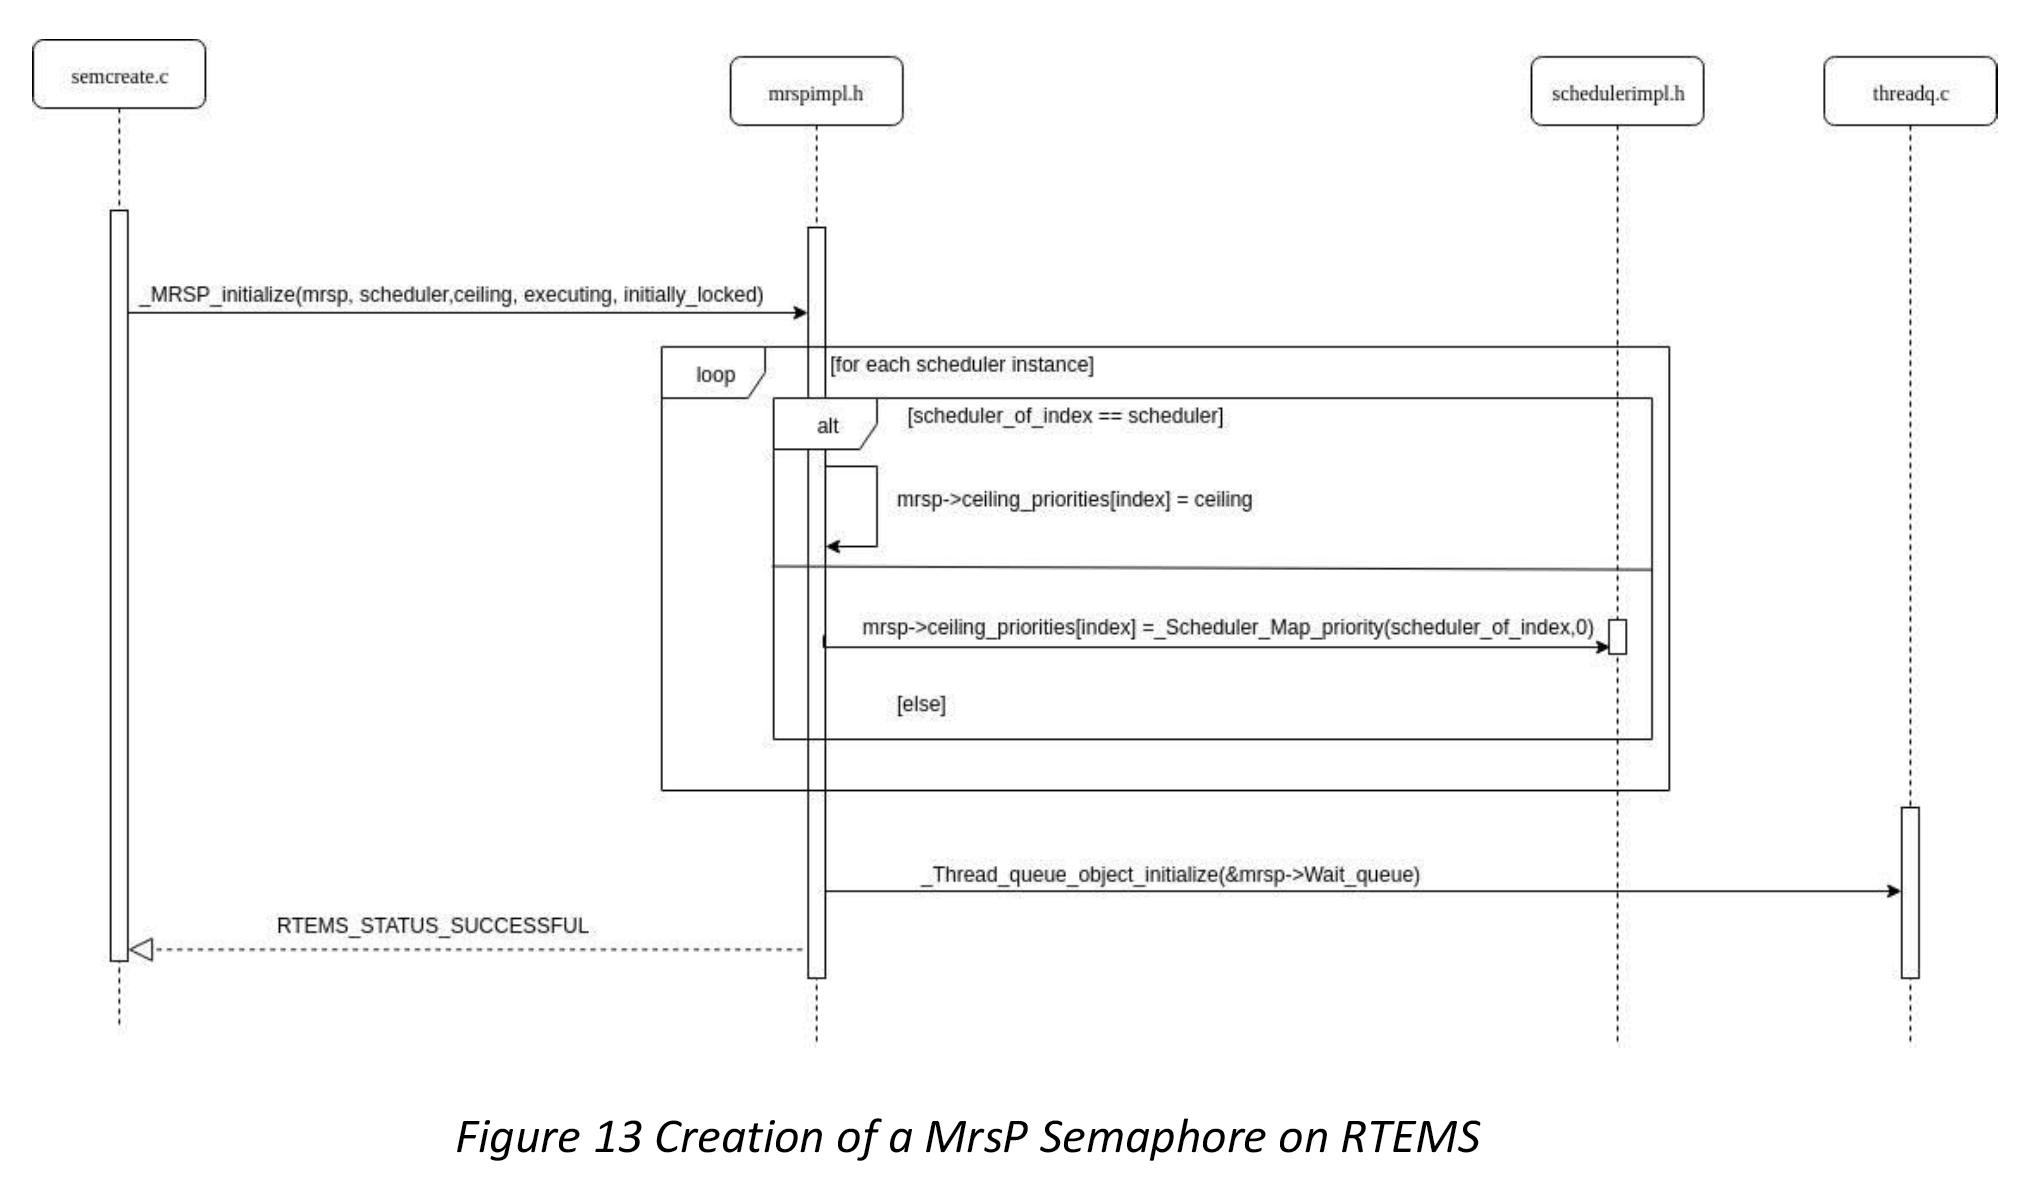
\includegraphics[width=\textwidth]{../images/create-MrsP-semaphore-Gomes-2019.png}

(p42) \textbf{How MrsP semaphores are initialised!}

\begin{quotation}
``
The sticky level of a task,
when incremented to at least the value of 1,
grants that when the task is executing
in any scheduler instance other than its original one,
lower priority tasks may not execute on its host scheduler,
with the purpose of securing this property.
This feature is quite relevant,
according to the properties of MrsP,
mentioned on chapter 3,
where it is defined that under semaphores using MrsP,
lower priority tasks must be
prevented from executing on the host processor of the holder of the resource.
'' (p45)
\end{quotation}


\textbf{Worth figuring out how to emulate the sets in Section 6}

\subsubsection{Appendix 2}

The purpose of \verb"_Thread_queue_Path_acquire_critical" is described here.


\subsection{Relevant code}


\appendix

% \newpage\input{../template.lc}

\end{document}
